\documentclass[]{article}
\usepackage[round]{natbib}

\usepackage[margin=1in]{geometry}
\usepackage{url}
\usepackage{authblk}
\usepackage{graphicx}
\usepackage{color}
\usepackage{xspace}
\usepackage{amsmath,amssymb}
\usepackage{longtable,booktabs,array}
\usepackage{calc} % for calculating minipage widths
\usepackage[numbib]{tocbibind} % makes the references have a section number
\renewcommand{\bibname}{Supporting references}

% cross-reference with main text
\usepackage{xr}
\externaldocument{paper}

% external latex tables
\usepackage{catchfile}
\begin{filecontents*}{AFR.sd1.tex}
\end{filecontents*}


\begin{document}

\title{Supporting Information for\\
``Local fitness and epistatic effects lead to distinct patterns of linkage disequilibrium in protein-coding genes''}
\author[]{Aaron P. Ragsdale}
\affil[]{Department of Integrative Biology, University of Wisconsin--Madison, WI, USA}
\affil[]{apragsdale@wisc.edu}
\date{\today}
\maketitle

\renewcommand{\thefigure}{S\arabic{figure}}
\renewcommand{\thetable}{S\arabic{table}}
\renewcommand{\theequation}{S\arabic{equation}}
\renewcommand{\thesection}{S\arabic{section}}
\setcounter{figure}{0}
\setcounter{table}{0}
\setcounter{equation}{0}
\setcounter{section}{0}

\tableofcontents
\newpage

\clearpage

\section{The diffusion equation and moment system for the two-locus sampling distribution}

The two-locus diffusion equation with additive selection was first described by
\citet{Kimura1955-qe} and studied extensively in the 1960s and 70s (e.g.,
\citet{Hill1966-gv,Ohta1969-ie}). The continuous distribution \(\psi(x_1, x_2,
x_3)\) of haplotype frequencies in a population, where \(x_1\) is the frequency
of \(AB\), \(x_2\) of \(Ab\), and \(x_3\) of \(aB\), is governed by the
multi-dimensional Fokker-Planck equation:
\begin{align} \label{eq:diffeq}
\frac{\partial \psi}{\partial \tau} = &
\frac{1}{2}\mathop{\sum\sum}_{1\leq i, j \leq 3}
\frac{\partial^2}{\partial x_i \partial x_j}
\left[\frac{x_i(\delta_{i=j}-x_j)\psi}{\nu(\tau)}\right] \\\nonumber
& -\frac{\rho}{2}\left(-\frac{\partial}{\partial x_1} D\psi
  + \frac{\partial}{\partial x_2} D\psi
  + \frac{\partial}{\partial x_3} D\psi\right) \\\nonumber
& - \frac{\gamma_A}{2}\left[
  \frac{\partial}{\partial x_1} x_1(1-x_1-x_2)\psi
  + \frac{\partial}{\partial x_2} x_2(1-x_1-x_2)\psi
  - \frac{\partial}{\partial x_3} x_3(x_1+x_2)\psi
  \right] \\\nonumber
& -\frac{\gamma_B}{2}\left[
  \frac{\partial}{\partial x_1} x_1(1-x_1-x_3)\psi
  - \frac{\partial}{\partial x_2} x_2(x_1+x_3)\psi
  + \frac{\partial}{\partial x_3} x_3(1-x_1-x_3)\psi
  \right].
\end{align}
\(D\) is the standard covariance measure of linkage disequilibrium, \[D=x_1 -
(x_1+x_2)(x_1+x_3) = x_1 x_4 - x_2 x_3,\] \(\gamma_A\) and \(\gamma_B\) are the
(additive) scaled selection coefficients at the left and right locus, and
\(\rho\) is the scaled recombination rate between the two loci. Time \(\tau\) is
measured in \(2N_e\) generations, and \(\nu(\tau)\) is the population size relative
to the ancestral size or some reference size at time \(\tau\).

Given a function \(\psi\) that solves Equation \ref{eq:diffeq}, the two-locus
sampling distribution for a sample size of \(n\) haploids can be found by
integrating \(\Psi\) against the multinomial sampling function, so that
\begin{align} \label{eq:multinomial}
\Psi_n(i, j, k) =
{n \choose{i, j, k, n-i-j-k}}
\mathop{\mathop{\int\int\int}_{x_1, x_2, x_3 \geq0}}_{x_1+x_2+x_3\leq1}
\psi(x_1, x_2, x_3) x_1^i x_2^j x_3^k (1-x_1-x_2-x_3)^{n-i-j-k}
dx_1 dx_2 dx_3.
\end{align}

In the method-of-moments approach, instead of solving the differential equation
for \(\psi\), we instead integrate both sides of the differential equation
against the multinomial sampling function for a given sampling configuration
\((i, j, k)\). On the left side, we get \(\partial_t \Psi_n(i, j, k)\), and on the
right we obtain, after some simple integration by parts and somewhat tedious
simplification, terms for drift, recombination, and selection that can be
written as sparse linear operators of \(\Psi_n\). Written compactly, this takes
the form
\begin{equation}
\partial_\tau \Psi_n =
\frac{1}{2\nu(\tau)}\mathcal{D}_{n}\Psi_n
+ \frac{\rho}{2}\mathcal{R}_{n}\Psi_n
+ \frac{\theta}{2}\mathcal{U}_{n}\Psi_n
+ \mathcal{S}_{n, \boldsymbol{\gamma}, \mathbf{h}}\Psi_n.
\end{equation}.

Alternatively, we arrive at this same linear system of equations by tracking
the expected sampling distribution over \(n\) lineages within the full population
and how that changes over time by drawing lineages from one generation to the
next in the style of \citet{Wright1931-wy}. Both \citet{Jouganous2017-pq}, for the
single-locus SFS, and \citet{Ragsdale2019-nt} drew this connection in detail, so I
refer readers to those previous papers for a fuller description of those
derivations and discussion. In the next section I simply repeat the results for
\(\mathcal{D}\), \(\mathcal{R}\), and \(\mathcal{U}\), briefly describe the moment
closure approximation (which is the same as presented in \citet{Ragsdale2019-nt}), and
then describe the selection operator \(\mathcal{S}\) for selection with
epistasis, both with and without dominance.

\subsection{Drift, mutation, recombination, and moment closure}

\subsubsection{Drift}

Drift for an entry \((i, j, k)\) depends only on \(\Psi_n\) and therefore closes.
The entries of \(\mathcal{D}\) are found by considering the possibility of a
coalescence event occurring within a given generation within \(n\) lineages in
the full population. If \(n \ll N\), we can safely assume that at most a single
such event occurs in any given generation.

\begin{align}
\mathcal{D}_{n}(i, j, k)\Psi_n =
& (i - 1) (n - i - j - k + 1) \Psi_n(i - 1, j, k) \\\nonumber
& + (i + 1) (n - i - j - k - 1) \Psi_n(i + 1, j, k) \\\nonumber
& + (i - 1) (k + 1) \Psi_n(i - 1, j, k + 1) \\\nonumber
& + (i + 1) (k - 1) \Psi_n(i + 1, j, k - 1) \\\nonumber
& + (i - 1) (j + 1) \Psi_n(i - 1, j + 1, k) \\\nonumber
& + (i + 1) (j - 1) \Psi_n(i + 1, j - 1, k) \\\nonumber
& + (j - 1) (n - i - j - k + 1) \Psi_n(i, j - 1, k) \\\nonumber
& + (j + 1) (n - i - j - k - 1) \Psi_n(i, j + 1, k) \\\nonumber
& + (j - 1) (k + 1) \Psi_n(i, j - 1, k + 1) \\\nonumber
& + (j + 1) (k - 1) \Psi_n(i, j + 1, k - 1) \\\nonumber
& + (k - 1) (n - i - j - k + 1) \Psi_n(i, j, k - 1) \\\nonumber
& + (k + 1) (n - i - j - k - 1) \Psi_n(i, j, k + 1) \\\nonumber
& - 2\left( i ( n - i - j - k) + i k + i j + j (n - i - j - k) + j k + k(n - i - j - k)\right)\Psi_n(i, j, k)
\end{align}

\subsubsection{Recombination}

If a lineage in our sample of size \(n\) recombines in a given generation, which
occurs with probability \(nr\), we need to draw an extra lineage from the full
population for it to recombine with. This means we need \(\Psi_{n+1}\) in the
previous generation. After drawing that extra lineage, \(\Psi_n\) changes as we
draw one of the two recombinant types (each with probability \(1/2\)) instead of
the lineage that was chosen to recombine.

\begin{align}
\mathcal{R}_{n}(i, j, k)\Psi_n = &
\frac{(i + 1)(n - i - j - k + 1)}{n + 1}\Psi_{n+1}(i + 1, j - 1, k) \\\nonumber
& + \frac{(i + 1)(n - i - j - k + 1)}{n + 1}\Psi_{n+1}(i + 1, j, k - 1) \\\nonumber
& + \frac{(j + 1)(k + 1}{n + 1)}\Psi_{n+1}(i - 1, j + 1, k + 1) \\\nonumber
& + \frac{(j + 1)(k + 1}{n + 1)}\Psi_{n+1}(i, j + 1, k + 1) \\\nonumber
& - \frac{(i + 1)(n - i - j - k)}{n + 1}\Psi_{n+1}(i + 1, j, k) \\\nonumber
& - \frac{(j + 1) k}{n + 1}\Psi_{n+1}(i, j + 1, k) \\\nonumber
& - \frac{j (k + 1)}{n + 1}\Psi_{n+1}(i, j, k + 1) \\\nonumber
& - \frac{i (n - i - j - k + 1}{n + 1}\Psi_{n+1}(i, j, k)
\end{align}

\subsubsection{Mutation}

We assume an infinite sites mutation (ISM) model where new mutations occur at
previously unmutated loci. In the two-locus ISM model, two-locus pairs of
variable loci arise when a mutation occurs at one locus when the other locus is
already variable. Thus, new mutations at the \(B/b\) locus occur against the
single-locus allele frequency distribution \(\Phi_{n,A}\), and new mutations at
the \(A/a\) locus occur against \(\Phi_{n, B}\), which are found via the single-locus
system from \citet{Jouganous2017-pq}.

\begin{align}
\mathcal{U}_{n}(i, j, k)\Psi_n = &
(j + 1)\frac{\theta_B}{2} \Phi_{n, A}(j+1) \delta_{i=1, k=0} \\\nonumber
& + (n - j)\frac{\theta_B}{2} \Phi_{n, A}(j) \delta_{i=0, k=1} \\\nonumber
& + (i + 1)\frac{\theta_A}{2} \Phi_{n, B}(i+1) \delta_{i=1, j=0} \\\nonumber
& + (n - i)\frac{\theta_A}{2} \Phi_{n, B}(i) \delta_{i=0, j=1} \\\nonumber
\end{align}

\subsubsection{Jackknife moment closure approximation}\label{jackknife-moment-closure-approximation}

We use a jackknife approximation to write the entries of \(\Psi_{n+1}\) and
\(\Psi_{n+2}\) as linear combinations of entries in \(\Psi_n\). The general
strategy is to assume the underlying continuous distribution \(\psi(x_1, x_2, x_3)\) can be approximated locally as a quadratic, and then use entries in
\(\Psi_n\) that are close in frequency to a given entry in \(\Psi_{n+l}\) to
estimate the coefficients of that quadratic using the multinomial sampling
formula. Then this quadratically local approximation to \(\psi\) can be used to
compute \(\Psi_{n+l}(i, j, k)\) using Eq. \eqref{eq:multinomial}. Readers should
refer to section S1.3.5 in the Supporting material for \citet{Ragsdale2019-nt} for
details.

\subsection{Selection}

First consider the case of no dominance, so that the haplotypes \(Ab\), \(aB\),
and \(AB\) have selection coefficients \(s_{Ab}\), \(s_{aB}\), and \(s_{AB}\),
respectively. Note that the case with \(s_{AB} = s_{Ab} + s_{aB}\) implies no
epistasis between the \(A/a\) and \(B/b\) loci. Here, we assume all selection
coefficients are negative. In a given generation, a selection event could
occur in which a haplotype is rejected (selected against) with probability
proportional to its selection coefficient, \(-s\). We then draw an extra lineage
from the full population to replace that rejected lineage.

For example, the probability that an \(AB\) haplotype is selected against and
replaced by an \(Ab\) haplotype is \[-ns_{AB} \frac{i}{n+1}{j+1}{n}\Psi_{n+1}(i,
j + 1, k),\] where the additional \(j + 1\) lineage in a sample of size \(n + 1\)
accounts drawing that extra \(Ab\) haplotype. Taking all such selective events
together, for additive selection we get
\begin{align}
\mathcal{S}_{n}(i, j, k)\Psi_n = &
\frac{i+1}{n+1}\left(-s_{AB}(n-i) + s_{Ab}j
+ s_{aB}k\right)\Psi_{n+1}(i+1, j, k) \\\nonumber
& +\frac{j+1}{n+1}\left(s_{AB}i - s_{Ab}(n-j)
+ s_{aB}k\right)\Psi_{n+1}(i, j+1, k) \\\nonumber
& +\frac{k+1}{n+1}\left(s_{AB}i + s_{Ab}j
- s_{aB}(n-k)\right)\Psi_{n+1}(i, j, k+1) \\\nonumber
& + \frac{n-i-j-k+1}{n+1}\left(s_{AB}i + s_{Ab}j
+ s_{aB}k\right)\Psi_{n+1}(i, j, k)
\end{align}

For a general diploid selection model, the idea is nearly the same, but we need
to draw an extra lineage to determine the fitness of a diploid individual. For
example, the probability that an \(AB\) haplotype is paired with an additional
lineage \(Ab\) and selected against, and then replaced by an \(aB\) haplotype is
\[-ns_{AB/Ab}\frac{i}{n+2}\frac{j+1}{n+1}\frac{k+1}{n}\Psi_{n+2}(i, j+1,
k+1).\] There are now many more possible selective events to consider, but
after accounting for all possible diploid pairs and replacements (90 in total)
and simplifying, we find

\begin{align}
\mathcal{S}_{n}(i, j, k)\Psi_n = &
\frac{n-i-j-k+2}{n+2}\frac{n-i-j-k+1}{n+1}\left(
  s_{AB/ab}i
  + s_{Ab/ab}j
  + s_{aB/ab}k
\right)\Psi_{n+2}(i,j,k) \\\nonumber
& + \frac{i+1}{n+2}\frac{n-i-j-k+1}{n+1}(
  s_{AB/AB}i
  + s_{AB/Ab}j
  + s_{AB/aB}k
  + s_{Ab/ab}j \\\nonumber & \hspace{20pt}
  + s_{aB/ab}k
  - s_{AB/ab}(n + j + k)
)\Psi_{n+2}(i+1, j, k) \\\nonumber
& + \frac{i+2}{n+2}\frac{i+1}{n+1}(
  s_{AB/Ab}j
  + s_{AB/aB}k
  + s_{AB/ab}(n-i-j-k)
  - s_{AB/AB}(n-i)
)\Psi_{n+2}(i+2, j, k) \\\nonumber
& + \frac{i+1}{n+2}\frac{j+1}{n+2}(
  s_{AB/AB}i
  + s_{AB/aB}k
  + s_{AB/ab}(n-i-j-k)
  + s_{Ab/Ab}j \\\nonumber & \hspace{20pt}
  + s_{Ab/aB}k
  + s_{Ab/ab}(n-i-j-k)
  - s_{AB/Ab}(2n-i-j)
)\Psi_{n+2}(i+1, j+1, k) \\\nonumber
& + \frac{i+1}{n+2}\frac{k+1}{n+1}(
  s_{AB/AB}i
  + s_{AB/Ab}j
  + s_{AB/ab}(n-i-j-k)
  + s_{Ab/aB}j \\\nonumber & \hspace{20pt}
  + s_{aB/aB}k
  + s_{aB/ab}(n-i-j-k)
  - s_{AB/aB}(2n-i-k)
)\Psi_{n+2}(i+1, j, k+1) \\\nonumber
& + \frac{j+1}{n+2}\frac{n-i-j-k+1}{n+1}(
  s_{AB/Ab}i
  + s_{AB/ab}i
  + s_{Ab/Ab}j
  + s_{Ab/aB}k \\\nonumber & \hspace{20pt}
  + s_{aB/ab}k
  -s_{Ab/ab}(n+i+k)
)\Psi_{n+2}(i, j+1, k) \\\nonumber
& + \frac{j+2}{n+2}\frac{j+1}{n+1}(
s_{AB/Ab}i + s_{Ab/aB}k + s_{Ab/ab}(n-i-j-k) - s_{Ab/Ab}(n-j)
)\Psi_{n+2}(i, j+2, k) \\\nonumber
& + \frac{j+1}{n+2}\frac{k+1}{n+1}(
  s_{AB/Ab}i
  + s_{AB/aB}i
  + s_{Ab/Ab}j
  + s_{Ab/ab}(n-i-j-k) \\\nonumber & \hspace{20pt}
  + s_{aB/aB}k
  + s_{aB/ab}(n-i-j-k)
  - s_{Ab/aB}(2n - j - k)
)\Psi_{n+2}(i, j+1, k+1) \\\nonumber
& + \frac{k+1}{n+2}\frac{n-i-j-k+1}{n+1}(
  s_{AB/aB}i
  + s_{AB/ab}i
  + s_{Ab/aB}j
  + s_{Ab/ab}j \\\nonumber & \hspace{20pt}
  + s_{aB/aB}k
  - s_{aB/ab}(n + i + j)
)\Psi_{n+2}(i, j, k+1) \\\nonumber
& + \frac{k+2}{n+2}\frac{k+1}{n+1}(
  s_{AB/aB}i
  + s_{Ab/aB}j
  + s_{aB/ab}(n-i-j-k)
  - s_{aB/aB}(n - k)
)\Psi_{n+2}(i, j, k+2).
\end{align}
Multiplying through by \(2N_{ref}\) gives us selection operators in terms of
\(\gamma\) instead of \(s\).

\subsection{Validation against simulation}

To assess the accuracy of the numerical approximation, I carried out discrete
two-locus simulations over a range of recombination rates and selection
parameterizations. Such discrete simulations track allele and haplotype
frequencies in a population of a given size, with offspring generations
constructed via multinomial sampling from the haplotype frequencies in the
parental generation. Because we only track the two focal loci, these
simulations do not contain any additional effects of linked selection (see
Section~\ref{sec:bgs} for simulations with many linked loci).

Simulations had diploid population sizes of 5000 and I drew haploid sample
sizes of 50 (25 diploids), with recombination rates varying from \(0\) to
\(0.001\) (or \(\rho=0-20\)). I tested selection coefficients of \(s\) of 0,
\(-1\times10^{-5}\), \(-2\times10^{-4}\), and \(-2\times10^{-3}\) (or
\(\gamma=0\), \(-0.1\), \(-2\), and \(-20\)). Epistasis was set to
\(\epsilon=0\), \(-0.5\), and \(0.5\), and dominance was set to either
\(h=0.5\) (additive) or \(0.1\) (recessive). Conditional distributions of the
two-locus sampling distribution show good agreement between numerical solutions
and simulations, and residuals do not show any directional bias
(Figures~\ref{fig:validation1}--\ref{fig:validation5}). The Supporting Figures
includes a handful of these comparisons, and the full set of comparisons (over
40 in total across the range of parameters listed above), simulation, and
plotting scripts in Python are available at
\url{https://github.com/apragsdale/two_locus_selection}.

To assess the accuracy under dominance, I simulated under the
\citet{Roze2021-cf} scenarios (\(N=1000\), \(r=0.0001\) and \(0.001\), and
\(sh=-0.0001\), \(-0.0004\), \(-0.001\), and \(-0.01\)). Note that \(sh=-0.01\)
is extremely strong selection, especially for small \(h\), and \texttt{moments}
was unstable in that parameter regime. For weak and moderate selection, there
good agreement between simulated data and \texttt{moments} solutions
(Figure~\ref{fig:dominance}D, E).

\subsection{Background selection and associative overdominance}\label{sec:bgs}

To explore the effects of many linked selected loci on patterns of LD, I used
\texttt{fwdpy11} \citep{Thornton2014-pn,Thornton2019-qc} to simulate large
genomic segments with many selected mutations. Each simulation had population
size of \(N=1000\), a sequence length of 1Mb, with mutation and recombination
rates both \(u=r=10^{-8}\). I considered four scenarios for selected mutations:
additive selection \(h=0.5\) with \(s=-0.0005\) and \(s=-0.01\) (\(\gamma=-1\)
and \(-20\)), and recessivity \(h=0.0\) or \(h=0.1\) with the same selection
coefficients. These sets of parameters should give rise to strong effects of
linked selection, as there are many cosegregating, tightly linked selected
variants. For each setting, I examined site-frequency spectra and LD decay for
both selected and neutral mutations across the region.

For each simulation, I ran a large number of replicates (100 independent
replicates, and within each replicate, I sampled 25 diploid individuals every
100 generations for a total of 20,000 samples from each replicate, after
burn-in of \(100N\) generations). Additive selection caused minor distortions
to the SFS, and reduced observed \(\sigma_d^1\) and \(\sigma_d^2\) in the case
of weak selection (\(\gamma=-1\)) (Figure~\ref{fig:bgs1}). LD was largely
unaffected in the stronger selection scenario, consistent with intuition that
interference (including interference from additional linked sites) is most
noticeable for \(s\approx1/N\) (Figure~\ref{fig:bgs2}).

Larger deviations from two-locus expectations were observed for recessive
mutations. For recessive weakly deleterious mutations (Figure~\ref{fig:bgs3}),
there is a large excess of neutral and selected mutations at common frequencies
(due to associative overdominance \citep{Zhao2016-bb}). \(\sigma_d^2\) for
neutral and selected mutations is also increased over two-locus expectations.
Stronger recessive mutations (Figure~\ref{fig:bgs4}) also show distorted allele
frequencies, though the distortion to LD is not as strong as observed for weak
recessive variants.

\subsection{Frequency dependence of signed LD}

Mutations at different frequencies are expected to have different signs and
magnitudes of LD. For example, rare mutations show highly positive LD, even for
pairs of neutral mutations \citep{Good2022-ot}. Mutations of different
functional classes (synonymous, missense, and loss-of-function, for example)
are expected to segregate at different average frequencies, and average
selection pressures are observed to be greater within annotated conserved
domains, with stronger purifying selection driving allele frequencies to
relatively lower levels among missense and loss-of-function variants. Since
mutations of difference classes and locations have different average
frequencies, this may drive differences in patterns of LD when comparing
between them.

One approach to lessen the impact of differing allele frequencies when
comparing between classes of mutations is to condition on allele frequencies.
From sampling data with observed derived allele counts, it is simplest to
condition on those allele counts \citep[e.g.,\(n_A,n_B=2\),][]{Garcia2021-zn},
and to compute \(\sigma_d^1\) and \(\sigma_d^2\) from pairs of mutations that
satisfy that condition. In the simulations with haploid sample sizes \(n=50\)
(Figures~\ref{fig:toy},~\ref{fig:relate_dom},~\ref{fig:toy_sd2}--\ref{fig:relate_dom_sd2}),
I partitioned allele counts as uncommon (\(n_A, n_B \leq 4\), or \(\hat{f_A},
\hat{f_B} \leq 0.08\)), or common (\(n_A, n_B \geq 5\)). In the
\citet{1000_Genomes_Project_Consortium2015-zq} data, in which most populations
have diploid sample sizes between 80 and 100, I considered \(n_A, n_B \geq 2\),
\(3\leq n_A, n_B \leq 8\), and \(n_A, n_B \geq 9\) (or rare, uncommon, and
common (\(\gtrsim 0.05\))). Functions to compute allele-count-conditioned
statistics from \(\Psi_n\) are packaged within \texttt{moments}.

\section{Data analysis}

\subsection{DFE for missense and LOF variants}

Loss-of-function (LOF) variants show a dramatic skew toward low-frequency
variants across all human populations (Table \ref{tab:tajimasD}). Here, using
the folded SFS for synonymous, missense, and LOF mutations across all autosomal
genes, I inferred DFEs for missense and LOF mutations independently. I
considered a few different dominance coefficients to explore the effect of the
assumed recessivity of the two classes of mutations.

The standard SFS approach to fitting the DFE involves first inferring a
demographic history for the population using putatively neutral variants (here,
synonymous mutations), and then fixing that demography and fitting a
parameterized function for the distribution of selection coefficients for new
mutations for the selected classes. DFE inference also requires an estimate for
the total mutation rate of the different mutation classes, as much of the
signal for strongly selected mutations comes from observing fewer mutations
than expected given a known mutation rate (with the assumption that selection
purges some fraction of strongly deleterious mutations which are unseen in the
sample). Here, I fit demography and DFEs to the folded SFS from the Mende in
Sierra Leone (MSL) using \emph{moments} version 1.1.0 \citep{Jouganous2017-pq}.

I used the mutation model from \citet{Karczewski2020-le} to estimate the total
mutation rate across autosomal genes (\(uL\), where \(u\) is the per-base
mutation rate of a given mutation class, and \(L\) is the total length of the
coding genome). These values were \((0.1442, 0.3426, 0.0256)\) for synonymous,
missense, and LOF mutations, respectively. Roughly two thirds of new mutations
in coding regions are expected to be missense mutations, while only 5\% of new
mutations are LOF. I fit a demographic model to the synonymous variants, which
included a population expansion in the deeper past and exponential growth in
the recent past (Figure \ref{fig:msldemogdfe}A). Using the inferred optimal
scaled mutation rate, \(\theta=4N_euL\), I estimated \(Ne\approx12,300\), and
assuming an average generation time of 29 years I converted the inferred
genetic units to physical units. The best-fit model had a roughly two-fold
expansion 400 thousand years ago, and then exponential growth over the past
20-30 thousand years, with a current effective size of \(\approx 63,000\).

Under this demographic model, I fit a gamma distribution for the distribution
of fitness effects to missense and LOF mutations (Table \ref{tab:msldfe}). For
each fit, I fixed the scaled mutation rate for each mutation class, so that
\(\theta_{mis} = \frac{u_{mis}}{u_{syn}} \hat\theta_{syn}\) and \(\theta_{lof}
= \frac{u_{lof}}{u_{syn}} \hat\theta_{syn}\), where values of \(u\) were found
using the GNOMAD mutation model \citep{Karczewski2020-le}. I tested three
values for the dominance coefficient \(h\): \(0\), \(0.2\) and \(0.5\). For
missense mutations, \(h=0\) gave a poor fit to the data, and \(h=0.5\) fit best
among the three tested dominance coefficients. For LOF variants, \(h=0\) also
fit poorly, but \(h=0.2\) and \(h=0.5\) gave similar likelihoods, highlighting
that inferring dominance using the SFS is poorly constrained. Regardless of the
dominance coefficient assumed, however, the vast majority of LOF variants were
inferred to be strongly deleterious, with only \(\sim10\%\) of new mutations
having selection coefficients on the order \(1/N_e\) or less.

\subsection{Multinucleotide mutations and positive LD between linked synonymous variants}
\label{sec:mnm}

Multinucleotide mutations (MNMs) are complex mutational events that result in
multiple mutations occurring on the same haplotype background in a single
generation. Because MNMs fall on the same haplotype, those mutations will be in
positive LD, and LD between those pairs that are very tightly linked will not
be broken down all that rapidly. MNMs are expected to occur over relatively
short distances, on the order of 10s or 100s of base pairs, making them a
likely culprit of the observed positive LD among synonymous mutations at short
distances.

MNM events can be easily incorporated into the moment system with a simple
adjustment to the mutation operator. Instead of all mutations occurring
independently in haplotypes with mutations already segregating at the other
locus, some fraction of new mutations could instead occur spontaneously and
create a new pair of mutations with initial counts \(n_{AB}=1\) and
\(n_{ab}=n-1\). We can partition $\Psi_n$ into pairs of mutations due to MNM
events (\(\Psi_n^{MNM}\)) and those due to sequential mutation events
(\(\Psi_n^{ISM}\)), so that \(\Psi_n=\Psi_n^{MNM}+\Psi_n^{ISM}\). For given
scaled mutation rates \(\theta=4N_e\mu\), \(\Psi_n^{ISM}\propto\theta^2\) and
\(\Psi_n^{MNM}\propto p_{MNM}\theta\), where \(p_{MNM}\) is the probability
that a mutational event causes a multinucleotide mutation. This difference in
scaling means that \(\Psi_n\) is sensitive to both the overall mutation rate
\(\theta\) as well as the probability that a mutation is a MNM at a given
distance.

\subsubsection{Optimization details}

Here, I fit a simple exponential model for the fraction of new mutations at a
given distance that give rise to a MNM event, so that \(p_{MNM,d} = P(MNM | d)
= Ae^{-\lambda d}\), where \(d\) is the distance separating pairs of mutations
in base pairs. I considered all synonymous mutations within genes in the MSL
data and used the same population size history model as inferred in the DFE
section above for a demographic control. This left two parameters to be fit,
\(A\) and \(\lambda\), which I fit to the binned decay curve of \(\sigma_d^1\)
using the midpoint of each bin as the distance for that bin. I needed to assume
an average per-base recombination rate \(r\) across gene regions, and tested a
number of values between \(10^{-9}\) and \(2\times 10^{-8}\). Optimization was
insensitive to the chosen value of \(r\), because the decay of positive LD
occurs rapidly. For any plausible value of \(r\), \(\sigma_d^1\) decays to zero
well before distances between pairs have scaled recombination rates \(\rho=4
N_e r d \sim 1\), and expected statistics for \(\rho \ll 1\) vary negligibly.

To perform optimization, I assumed a Guassian likelihood function within each
bin using variances estimated via bootstrap replicates from sampling genes with
replacement. A composite likelihood was computed by taking the product of
likelihoods across bins. I used the estimate of \(Ne\approx12,300\) from the
DFE optimization using MSL data, a coding mutation rate of
\(\mu=1.33\times10^{-8}\) \citep{Karczewski2020-le}, and the fraction of coding
mutations that result in synonymous mutations was assumed to be (assuming a
ration of nonsynonymous mutations to synonymous mutations of 2.5:1). Thus, the
scaled mutation rate was \(\theta=4\times
N_e\times\mu\times\frac{1}{3.5}\approx1.87\times10^{-4}\).

\subsubsection{MNM optimization results and discussion}

In fitting the LD decay of \(\sigma_d^1\), the best fit parameters were
\(A=2.44\times10^{-5}\), and \(\lambda=0.00919\). Thus, only a small fraction
of new mutations were inferred to cause MNM events (\(\ll1\%\)), and
\(1/\lambda\approx 100\) means that the proportion of mutation events that
cause MNM decays quickly within a few hundred base pairs.

However, because of the differences in scaling of \(\Psi_n^{ISM}\) and
\(\Psi_n^{MNM}\) (with the square of \(\theta\) vs linearly as
\(p_{MNM}\theta\)), the number of \emph{observed} pairs of mutations at a given
distance that arose due to a MNM event is much larger. A rough estimate given
the assumed mutation rate and inferred parameters is that \(p_{MNM}\theta /
\theta^2 \approx 10\%\) of pairs of synonymous mutations observed at
\(d\approx0\) are due to MNM events, roughly \(p_{MNM}e^{-\lambda 100}\theta /
\theta^2 \approx 4\%\) at \(d=100\) base pairs, and only about
\(p_{MNM}e^{-\lambda 400}\theta / \theta^2 \approx 0.25\%\) at \(d=400\) base
pairs. This inference is very sensitive to the assumed mutation rate and the
proportion of mutations that cause synonymous vs nonsynonymous variants, and
future work will be needed to refine these estimates.

\subsection{Grouping Thousand Genomes populations based on clustering}

The large confidence intervals for measurements of signed LD could be driven by
either averaging over relatively few observed pairs of mutations, or due to
small sample sizes that make each individual measurement a noisy estimate of
the LD for that pair of mutations in the full population. To explore the
underlying cause of measurement uncertainty in the
\citet{1000_Genomes_Project_Consortium2015-zq} data, I considered larger sets of
samples by combining populations that consistently cluster together in PCA and
UMAP space and have low differentiation \citep{Diaz-Papkovich2020-ee}. I took
combinations of CEU/GBR, CHB/CHS, CDX/KHV, and MSL/GWD. While recognizing that
residual population structure in these population combinations could alter
expected LD statistics compared to the respective single-population estimates,
I was more interested in the effect that increasing the sample sizes would have
on estimated measurement error.

Across each of the four combinations tested, confidence intervals were roughly
equivalent to those of each of the individual populations. This suggests that
the limiting factor to accurate LD measurement is not sample size but rather
the overall levels of diversity and number of pairs of mutations that we
compare. \(\mathbb{E}[D]\) is most affected by common variants, and the sample
sizes of the Thousand Genomes Project data are likely sufficient to accurately
estimate common allele frequencies. Adding additional samples will increase the
number of rare variants that we observe, but rare variants have minimal impact
on \(\sigma_d^1\). Thus, the accuracy of estimates of \(\sigma_d^1\) is more
fundamentally limited by evolutionary history and genome biology (i.e.~past
population sizes, mutation and recombination rates) than by sample sizes.


\bibliographystyle{genetics}
\bibliography{paper}

\clearpage
\newpage

\section{Supporting tables}

\begin{table}[ht!]
    \centering
    \begin{tabular}{llll}
        \toprule
        Diploid genotype & General model & Simple dominance & Gene-based dominance\\
        \midrule
        $AB$ / $AB$ & $1 + s_{AB/AB}$ & $1 + 2s_A + 2s_B$ & $1 + 2s$\\
        $AB$ / $Ab$ & $1 + s_{AB/Ab}$ & $1 + 2s_A + 2s_Bh_B$ & $1 + 2s$\\
        $AB$ / $aB$ & $1 + s_{AB/aB}$ & $1 + 2s_Ah_A + 2s_B$ & $1 + 2s$\\
        $AB$ / $ab$ & $1 + s_{AB/ab}$ & $1 + 2s_Ah_A + 2s_Bh_B$ & $1 + 2sh$\\
        $Ab$ / $Ab$ & $1 + s_{Ab/Ab}$ & $1 + 2s_A$ & $1 + 2s$\\
        \addlinespace
        $Ab$ / $aB$ & $1 + s_{Ab/aB}$ & $1 + 2s_Ah_A + 2s_Bh_B$ & $1 + 2s$\\
        $Ab$ / $ab$ & $1 + s_{Ab/ab}$ & $1 + 2s_Ah_A$ & $1 + 2sh$\\
        $aB$ / $aB$ & $1 + s_{aB/aB}$ & $1 + 2s_B$ & $1 + 2s$\\
        $aB$ / $ab$ & $1 + s_{aB/ab}$ & $1 + 2s_Bh_B$ & $1 + 2sh$\\
        $ab$ / $ab$ & $1$ & $1$ & $1$\\
        \bottomrule
    \end{tabular}
    \caption{
        \textbf{General selection model for diploids and dominance models.}
        Different dominance and interactive effects can be implemented by
        assigning the appropriate values of $s$.
    }
    \label{tab:selmodels}
\end{table}


\begin{table}[ht!]
    \centering
    \begin{tabular}{ll}
        \toprule
        Haplotype & Fitness\\
        \midrule
        $AB$ & $(1 + s_A + s_B)(1+\epsilon)$\\
        $Ab$ & $1 + s_A$\\
        $aB$ & $1 + s_B$\\
        $ab$ & $1$\\
        \bottomrule
    \end{tabular}
    \caption{\textbf{Haploid epistasis model.}}
    \label{tab:epistasis}
\end{table}

\begin{table}[ht!]
    \centering
    \begin{tabular}{lll}
        \toprule
        Code & Description & Region\\
        \midrule
        ESN & Esan in Nigeria & Africa\\
        GWD & Gambian in Western Divisions in the Gambia & Africa\\
        LWK & Luhya in Webuye, Kenya & Africa\\
        MSL & Mende in Sierra Leone & Africa\\
        YRI & Yoruba in Ibadan, Nigeria & Africa\\
        \addlinespace
        CEU & Utah Residents (CEPH) with Northern and Western European Ancestry & Europe\\
        GBR & British in England and Scotland & Europe\\
        FIN & Finnish in Finland & Europe\\
        IBS & Iberian Population in Spain & Europe\\
        TSI & Toscani in Italia & Europe\\
        \addlinespace
        CDX & Chinese Dai in Xishuangbanna, China & East Asia\\
        CHB & Han Chinese in Beijing, China & East Asia\\
        CHS & Southern Han Chinese & East Asia\\
        JPT & Japanese in Tokyo, Japan & East Asia\\
        KHV & Kinh in Ho Chi Minh City, Vietnam & East Asia\\
        \bottomrule
    \end{tabular}
    \caption{
        \textbf{
            Thousand Genomes Project population descriptions
            for populations used in this study.
        }
    }
    \label{tab:1kgpops}
\end{table}

\begin{longtable}[t]{lllr}
\caption{\label{tab:tajimasD}
\textbf{Tamija's $D$ for classes of coding mutations.} Here, we partitioned by
synonymous, missense, and nonsense mutations, and considered all mutations gene-wide,
mutations falling within annotated conserved elements,
and mutations falling outside of those
elements.}\\
\toprule
Population & Mutation type & Region & Tajima's D\\
\midrule
\endfirsthead
\caption[]{\label{tab:tajimasD}Tamija's $D$ for classes of coding mutations.
\textit{(continued)}}\\
\toprule
Population & Mutation type & Region & Tajima's D\\
\midrule
\endhead

\endfoot
\bottomrule
\endlastfoot
ESN & Synonymous & All & -0.882\\
 &  & In domain & -0.854\\
 &  & Not in domain & -0.921\\
 & Missense & All & -1.414\\
 &  & In domain & -1.535\\
 &  & Not in domain & -1.293\\
 & Loss of function & All & -1.483\\
 &  & In domain & -2.156\\
 &  & Not in domain & -1.282\\
\addlinespace
GWD & Synonymous & All & -1.011\\
 &  & In domain & -0.981\\
 &  & Not in domain & -1.052\\
 & Missense & All & -1.566\\
 &  & In domain & -1.678\\
 &  & Not in domain & -1.452\\
 & Loss of function & All & -1.697\\
 &  & In domain & -2.328\\
 &  & Not in domain & -1.501\\
\addlinespace
LWK & Synonymous & All & -1.109\\
 &  & In domain & -1.088\\
 &  & Not in domain & -1.139\\
 & Missense & All & -1.589\\
 &  & In domain & -1.700\\
 &  & Not in domain & -1.477\\
 & Loss of function & All & -1.666\\
 &  & In domain & -2.278\\
 &  & Not in domain & -1.477\\
\addlinespace
MSL & Synonymous & All & -0.983\\
 &  & In domain & -0.959\\
 &  & Not in domain & -1.017\\
 & Missense & All & -1.501\\
 &  & In domain & -1.603\\
 &  & Not in domain & -1.400\\
 & Loss of function & All & -1.559\\
 &  & In domain & -2.303\\
 &  & Not in domain & -1.332\\
\addlinespace
YRI & Synonymous & All & -0.928\\
 &  & In domain & -0.898\\
 &  & Not in domain & -0.971\\
 & Missense & All & -1.467\\
 &  & In domain & -1.586\\
 &  & Not in domain & -1.348\\
 & Loss of function & All & -1.624\\
 &  & In domain & -2.237\\
 &  & Not in domain & -1.424\\
\addlinespace
CEU & Synonymous & All & -0.417\\
 &  & In domain & -0.392\\
 &  & Not in domain & -0.452\\
 & Missense & All & -1.248\\
 &  & In domain & -1.404\\
 &  & Not in domain & -1.082\\
 & Loss of function & All & -1.501\\
 &  & In domain & -2.196\\
 &  & Not in domain & -1.280\\
\addlinespace
FIN & Synonymous & All & -0.058\\
 &  & In domain & -0.047\\
 &  & Not in domain & -0.075\\
 & Missense & All & -0.883\\
 &  & In domain & -1.048\\
 &  & Not in domain & -0.710\\
 & Loss of function & All & -1.200\\
 &  & In domain & -2.034\\
 &  & Not in domain & -0.906\\
\addlinespace
GBR & Synonymous & All & -0.319\\
 &  & In domain & -0.300\\
 &  & Not in domain & -0.345\\
 & Missense & All & -1.120\\
 &  & In domain & -1.276\\
 &  & Not in domain & -0.954\\
 & Loss of function & All & -1.313\\
 &  & In domain & -2.178\\
 &  & Not in domain & -0.997\\
\addlinespace
IBS & Synonymous & All & -0.689\\
 &  & In domain & -0.664\\
 &  & Not in domain & -0.724\\
 & Missense & All & -1.424\\
 &  & In domain & -1.560\\
 &  & Not in domain & -1.279\\
 & Loss of function & All & -1.636\\
 &  & In domain & -2.349\\
 &  & Not in domain & -1.378\\
\addlinespace
TSI & Synonymous & All & -0.650\\
 &  & In domain & -0.625\\
 &  & Not in domain & -0.685\\
 & Missense & All & -1.422\\
 &  & In domain & -1.568\\
 &  & Not in domain & -1.266\\
 & Loss of function & All & -1.655\\
 &  & In domain & -2.349\\
 &  & Not in domain & -1.397\\
\addlinespace
CDX & Synonymous & All & -0.374\\
 &  & In domain & -0.366\\
 &  & Not in domain & -0.385\\
 & Missense & All & -1.179\\
 &  & In domain & -1.323\\
 &  & Not in domain & -1.026\\
 & Loss of function & All & -1.360\\
 &  & In domain & -2.194\\
 &  & Not in domain & -1.062\\
\addlinespace
CHB & Synonymous & All & -0.598\\
 &  & In domain & -0.593\\
 &  & Not in domain & -0.606\\
 & Missense & All & -1.389\\
 &  & In domain & -1.528\\
 &  & Not in domain & -1.239\\
 & Loss of function & All & -1.586\\
 &  & In domain & -2.344\\
 &  & Not in domain & -1.298\\
\addlinespace
CHS & Synonymous & All & -0.544\\
 &  & In domain & -0.545\\
 &  & Not in domain & -0.544\\
 & Missense & All & -1.334\\
 &  & In domain & -1.499\\
 &  & Not in domain & -1.150\\
 & Loss of function & All & -1.559\\
 &  & In domain & -2.290\\
 &  & Not in domain & -1.292\\
\addlinespace
JPT & Synonymous & All & -0.371\\
 &  & In domain & -0.368\\
 &  & Not in domain & -0.376\\
 & Missense & All & -1.194\\
 &  & In domain & -1.355\\
 &  & Not in domain & -1.019\\
 & Loss of function & All & -1.410\\
 &  & In domain & -2.272\\
 &  & Not in domain & -1.086\\
\addlinespace
KHV & Synonymous & All & -0.576\\
 &  & In domain & -0.562\\
 &  & Not in domain & -0.596\\
 & Missense & All & -1.346\\
 &  & In domain & -1.473\\
 &  & Not in domain & -1.210\\
 & Loss of function & All & -1.535\\
 &  & In domain & -2.294\\
 &  & Not in domain & -1.269\\*    
\end{longtable}

\begin{table}
    \centering
    \small
    \begin{tabular}{lrrrrrrrrr}
        \toprule
        Class & $h$ & shape & scale & LL &
        $[0,10^{-5})$ & $[10^{-5},10^{-4})$ & $[10^{-4},10^{-3})$ &
        $[10^{-3},10^{-2})$ & $[10^{-2},\infty)$\\
        \midrule
        Missense & 0.0 & 0.093 & 768505 & -678.2 & 0.260 & 0.062 & 0.077 & 0.096 & 0.505\\
         & 0.2 & 0.138 & 6660 & -416.7 & 0.260 & 0.098 & 0.134 & 0.182 & 0.327\\
         & 0.5 & 0.147 & 2117 & -392.0 & 0.282 & 0.114 & 0.159 & 0.214 & 0.231\\
        \addlinespace
        LOF & 0.0 & 0.132 & 99999054 & -248.3 & 0.077 & 0.028 & 0.037 & 0.051 & 0.807\\
         & 0.2 & 0.177 & 477994 & -226.7 & 0.083 & 0.042 & 0.063 & 0.095 & 0.717\\
         & 0.5 & 0.188 & 121419 & -224.2 & 0.092 & 0.050 & 0.077 & 0.119 & 0.662\\
        \bottomrule
    \end{tabular}
    \caption{
        \textbf{Distribution of fitness effects inferred for nonsynonymous mutations.}
        DFEs inferred for missense and loss-of-function variants in MSL for varying
        values of $h$. General patterns are consistent across different chosen values
        of $h$, although $h=0$ results in poorer fits for both missense and LOF variants.
        Columns to the right of the log-likelihood (LL) column show proportions of
        new mutations with $|s|$ in each given bin.
    }
    \label{tab:msldfe}
\end{table}

\CatchFileDef{\afrsigned}{AFR.sd1.tex}{}
\begin{table}
    \begin{center}
        \begin{tabular}{lccc}
            \afrsigned
        \end{tabular}
    \end{center}
    \caption{
        \label{tab:afrsd1}
        \textbf{Signed LD in AFR-labeled populations matched to distances
        and allele frequencies of synonymous mutations.}
        Gene-wide signed LD is observed to be at similar slightly positive levels between
        pairs of synonymous and pairs of missense variants. This observation is
        consistent when weighting missense variants to match distances between
        pairs of synonymous variants and when weighting to match synonymous allele
        frequencies, with only a slight reduction in missense \(\sigma_d^1\).
        The distribution of distances between synonymous and missense mutations
        within genes are very similar (Figure~\ref{fig:mutDistances}),
        so matching by distances separating mutations
        has a minor effect on measured average LD.
        The large measurement uncertainty of loss-of-function mutation pairs
        due to few observed pairs of such mutations within the same gene causes
        signed LD to fluctuate when conditioning on distances and frequencies
        matched to synonymous mutations.
    }
\end{table}

\CatchFileDef{\afrsquared}{AFR.sd2.tex}{}
\begin{table}
    \begin{center}
        \begin{tabular}{lccc}
            \afrsquared
        \end{tabular}
    \end{center}
    \caption{
        \label{tab:afrsd2}
        \textbf{Squared LD in AFR-labeled populations matched to distances
        and allele frequencies of synonymous mutations.}
    }
\end{table}

\CatchFileDef{\eursigned}{EUR.sd1.tex}{}
\begin{table}
    \begin{center}
        \begin{tabular}{lccc}
            \eursigned
        \end{tabular}
    \end{center}
    \caption{
        \label{tab:eursd1}
        \textbf{Signed LD in EUR-labeled populations matched to distances
        and allele frequencies of synonymous mutations.}
        Similar to the pattern observed in AFR-labeled populations
        (Table~\ref{tab:afrsd1}), \(sigma_d^1\) between missense mutations matched
        to distances and allele frequencies observed in synonymous mutation pairs
        has only a small effect on average signed LD, and gene-wide measurements
        are roughly equal between these two mutation classes.
        Again, measurement noise for loss-of-function mutation pairs is high.
    }
\end{table}

\CatchFileDef{\eursquared}{EUR.sd2.tex}{}
\begin{table}
    \begin{center}
        \begin{tabular}{lccc}
            \eursquared
        \end{tabular}
    \end{center}
    \caption{
        \label{tab:eursd2}
        \textbf{Squared LD in EUR-labeled populations matched to distances
        and allele frequencies of synonymous mutations.}
    }
\end{table}

\CatchFileDef{\eassigned}{EAS.sd1.tex}{}
\begin{table}
    \begin{center}
        \begin{tabular}{lccc}
            \eassigned
        \end{tabular}
    \end{center}
    \caption{
        \label{tab:eassd1}
        \textbf{Signed LD in EAS-labeled populations matched to distances
        and allele frequencies of synonymous mutations.}
        Similar to the pattern observed in AFR-labeled populations
        (Table~\ref{tab:afrsd1}), \(sigma_d^1\) between missense mutations matched
        to distances and allele frequencies observed in synonymous mutation pairs
        has only a small effect on average signed LD, and gene-wide measurements
        are roughly equal between these two mutation classes. 
        Again, measurement noise for loss-of-function mutation pairs is high.
    }
\end{table}

\CatchFileDef{\eassquared}{EAS.sd2.tex}{}
\begin{table}
    \begin{center}
        \begin{tabular}{lccc}
            \eassquared
        \end{tabular}
    \end{center}
    \caption{
        \label{tab:eassd2}
        \textbf{Squared LD in EAS-labeled populations matched to distances
        and allele frequencies of synonymous mutations.}
    }
\end{table}


\clearpage
\newpage

\section{Supporting figures}

\begin{figure}[ht!]
    \centering
    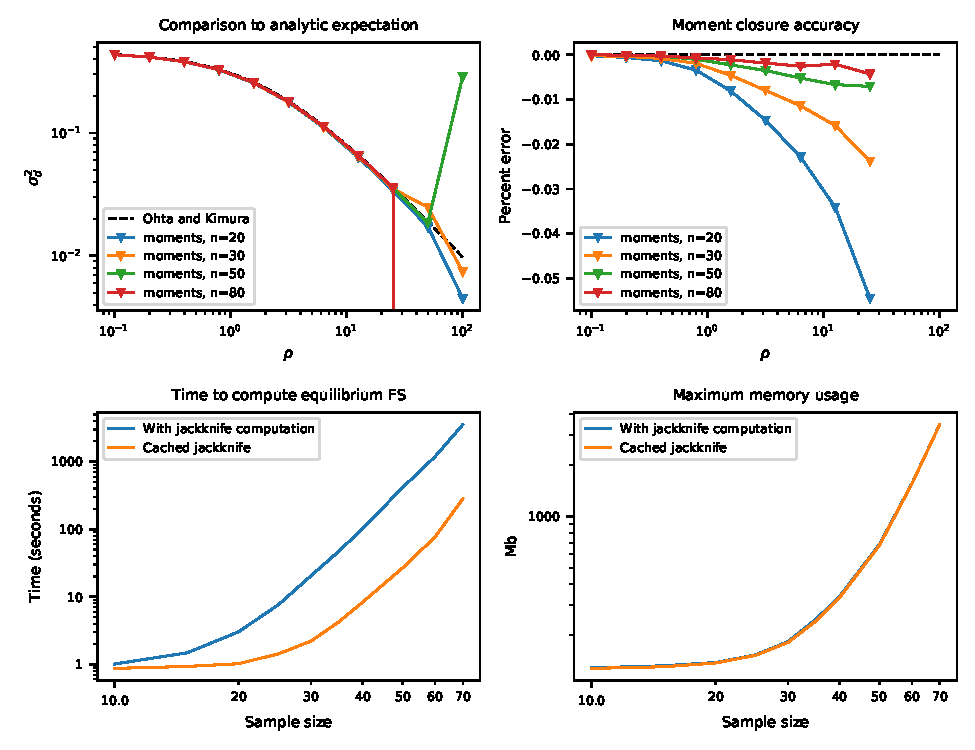
\includegraphics{../figures/jackknife}
    \caption{
        \textbf{Accuracy of the jackknife approximation and runtime.}
        Small sample sizes can lead to large error in the moment-closure
        approximation for larger recombination distances or selection
        coefficients. Generally, the jackknife approximation breaks down for
        recombination rates greater than \(\rho\gtrsim50\), depending on
        the sample size. While increasing
        sample size leads to more accurate solutions, it comes at the cost of
        both increased runtime and memory usage. Most analyses in this paper
        used sample sizes between 40 and 80.
    }
    \label{fig:jackknife}
\end{figure}

\begin{figure}[ht!]
    \centering
    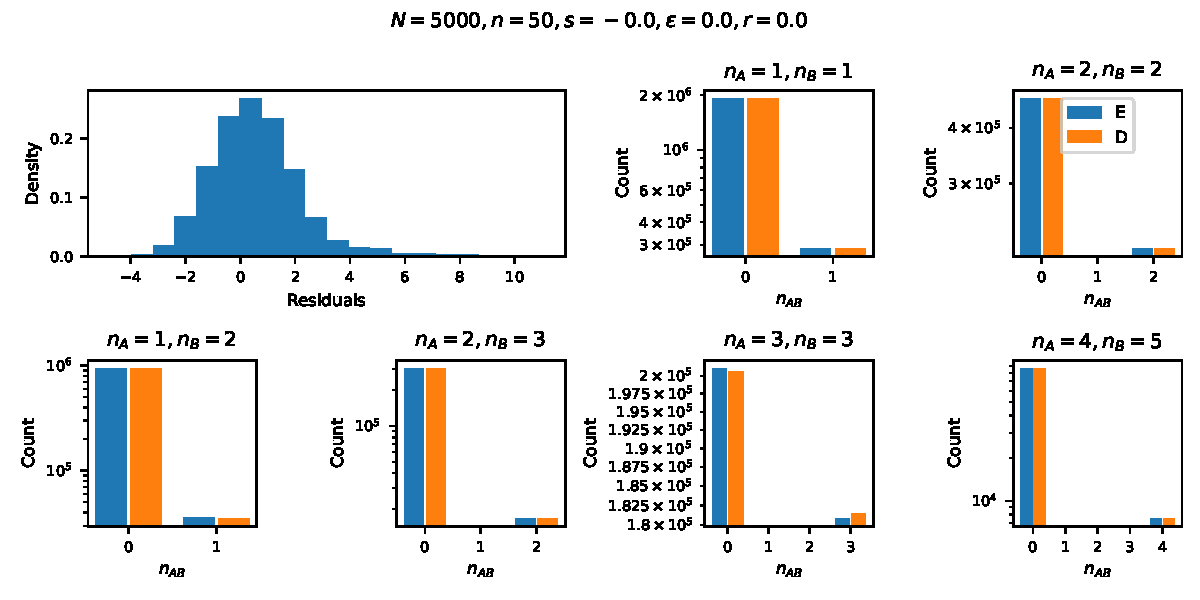
\includegraphics[width=\textwidth]{../simulations/discrete/plots/comp_Ne_5000_n_50_r_0.0_s_0.0_e_0.0.pdf}
    \caption{
        \textbf{Comparison between numerics and simulations for fully linked neutral loci.}
        With no recombination (\(r=0\)) and no selection, the moments solution is
        exact, and computing \(sigma_d^2\) from \(\Psi_n\) gives 5/11, the analytic
        solution from \citet{Ohta1969-ie}.
        Discrepancies between numerical expectations and the simulations are
        due to simulation noise, with Anscombe Poisson residuals roughly normally
        distributed around zero \citep{Pierce1986-um}.
        In the bar plots, ``E'' (blue) are expectations from \texttt{moments} and
        ``D'' are simulated data.
    }
    \label{fig:validation1}
\end{figure}

\begin{figure}[ht!]
    \centering
    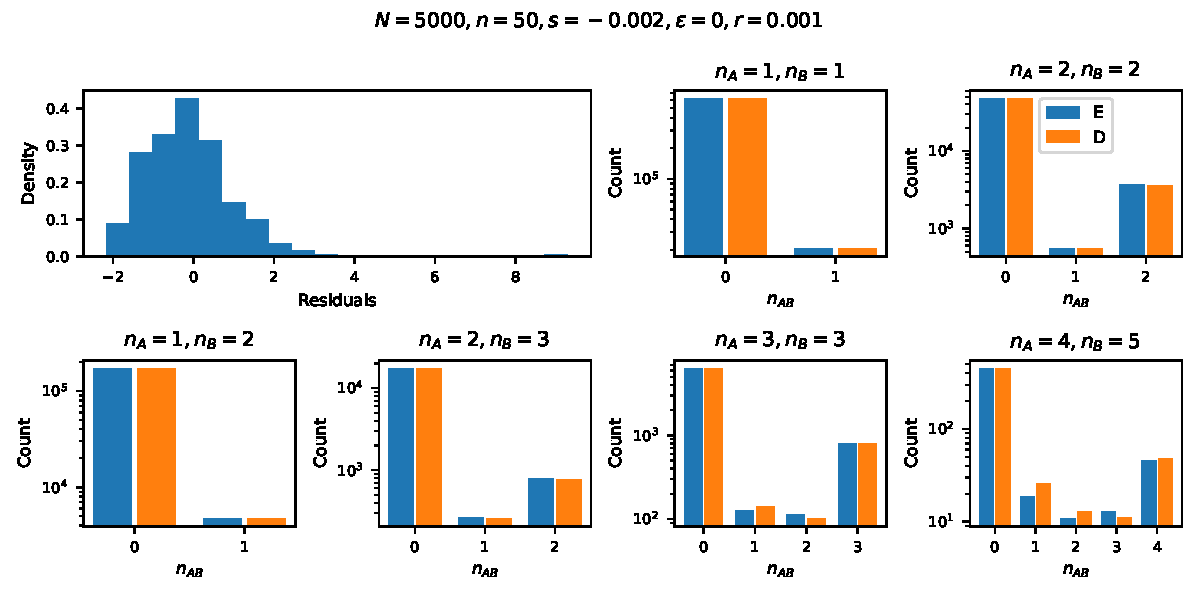
\includegraphics[width=\textwidth]{../simulations/discrete/plots/comp_Ne_5000_n_50_r_0.001_s_0.002_e_0.pdf}
    \caption{
        \textbf{Comparison to simulations for loosely linked additively selected loci.}
        \(Ne=5000\), \(r=0.001\), and \(s=-0.002\) (\(\rho=20\) and \(\gamma=-20\)
        at both loci), with no epistatic interactions (\(\epsilon=0\)).
        E: \texttt{moments} expectations, D: simulated data.
    }
    \label{fig:validation2}
\end{figure}

\begin{figure}[ht!]
    \centering
    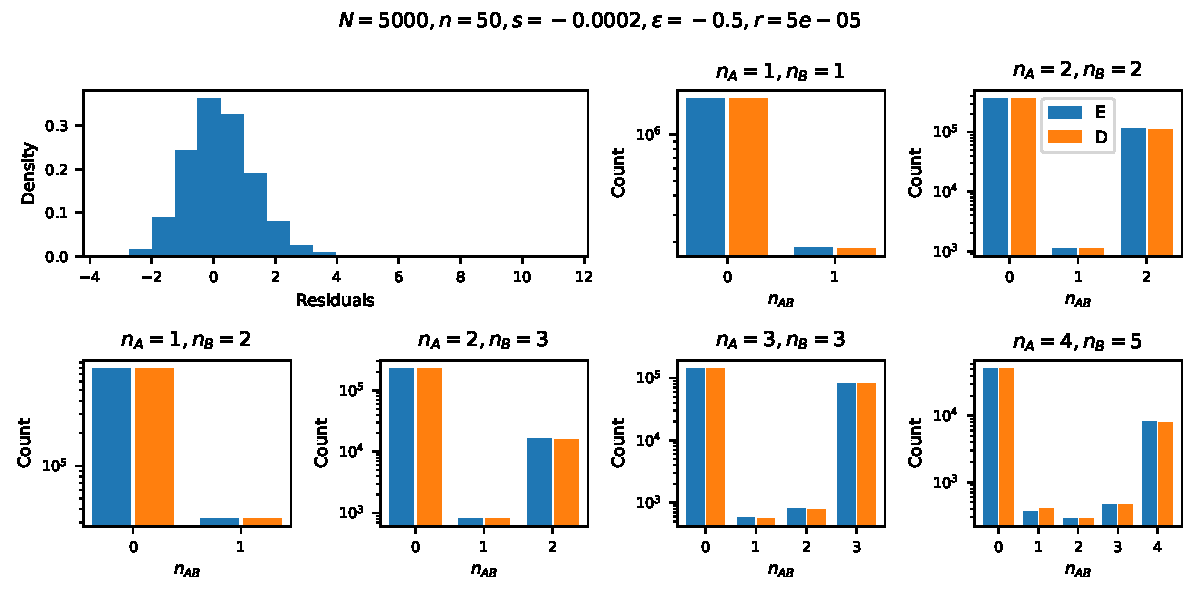
\includegraphics[width=\textwidth]{../simulations/discrete/plots/comp_Ne_5000_n_50_r_5e-05_s_0.0002_e_-0.5.pdf}
    \caption{
        \textbf{Comparison to simulations with antagonistic epistasis.}
        \(Ne=5000\), \(r=0.00005\), \(s=-0.0002\) (\(\rho=1\) and \(\gamma=-2\)
        at both loci), and \(\epsilon=-0.5\).
        E: \texttt{moments} expectations, D: simulated data.
    }
    \label{fig:validation3}
\end{figure}

\begin{figure}[ht!]
    \centering
    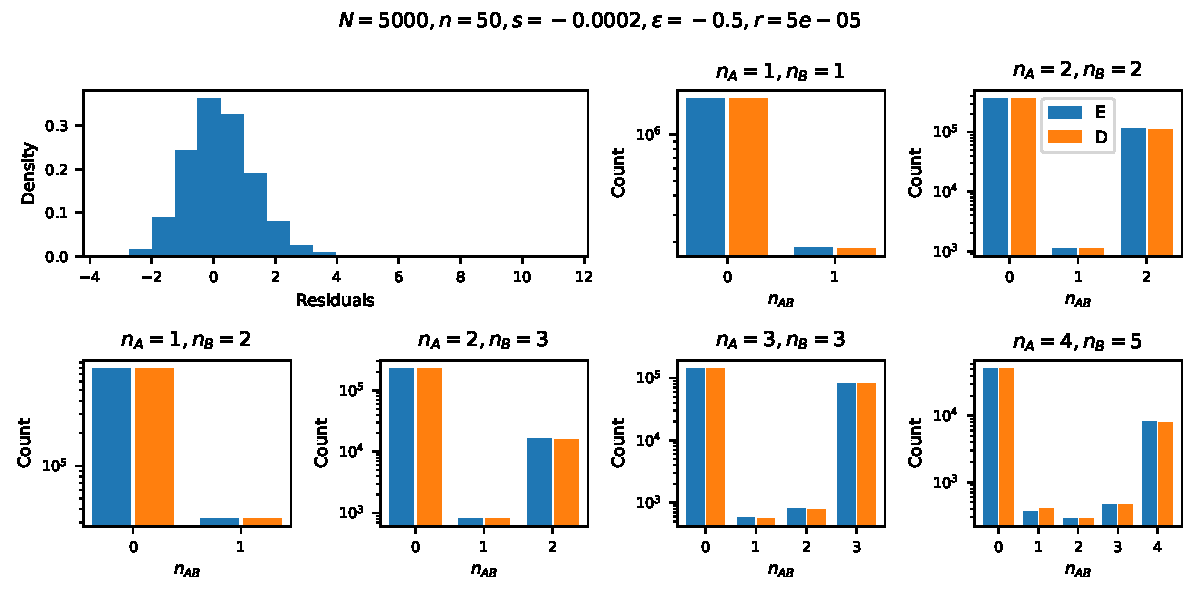
\includegraphics[width=\textwidth]{../simulations/discrete/plots/comp_Ne_5000_n_50_r_5e-05_s_0.0002_e_-0.5.pdf}
    \caption{
        \textbf{Comparison to simulations with synergistic epistasis.}
        \(Ne=5000\), \(r=0.00005\), \(s=-0.0002\) (\(\rho=1\) and \(\gamma=-2\)
        at both loci), and \(\epsilon=0.5\).
        E: \texttt{moments} expectations, D: simulated data.
    }
    \label{fig:validation4}
\end{figure}

\begin{figure}[ht!]
    \centering
    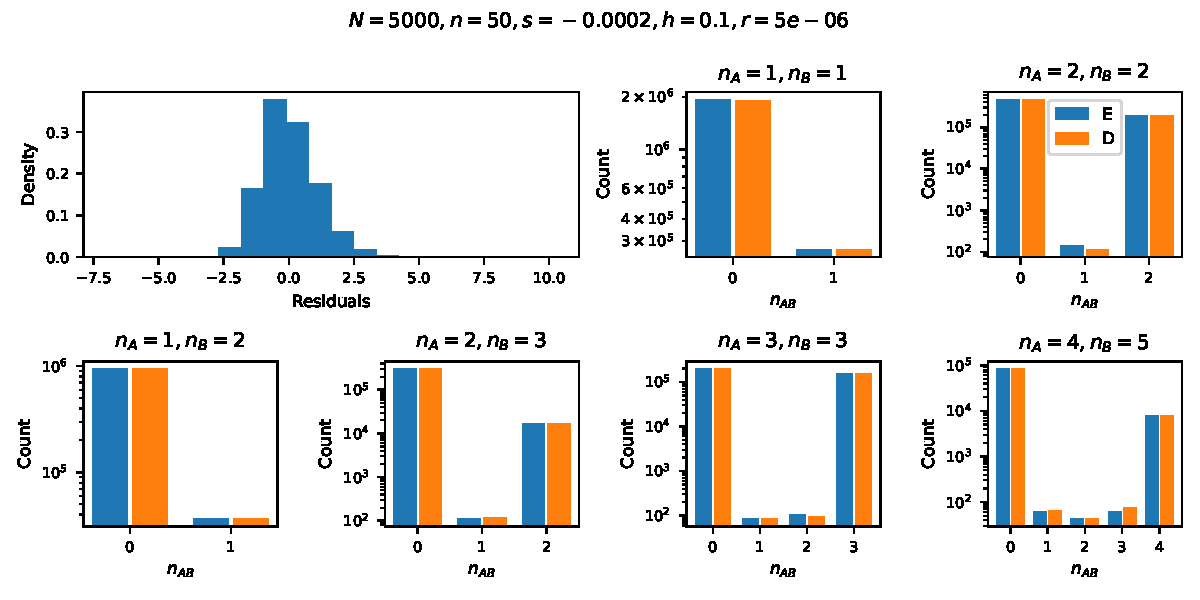
\includegraphics[width=\textwidth]{../simulations/discrete/plots/comp_Ne_5000_n_50_r_5e-06_s_0.0002_h_0.1.pdf}
    \caption{
        \textbf{Comparison to simulations with site-wise dominance.}
        \(Ne=5000\), \(r=5\times10^{-6}\), and \(s=-0.0002\) (\(\rho=0.1\) and
        \(\gamma=-2\)), with \(h=0.1\) at both loci and no
        epistatic interactions (\(\epsilon=0\)).
        E: \texttt{moments} expectations, D: simulated data.
        Additional comparisons to simulated data are available at
        \texttt{https://github.com/apragsdale/two\_locus\_selection}.
    }
    \label{fig:validation5}
\end{figure}

\begin{figure}[ht!]
    \centering
    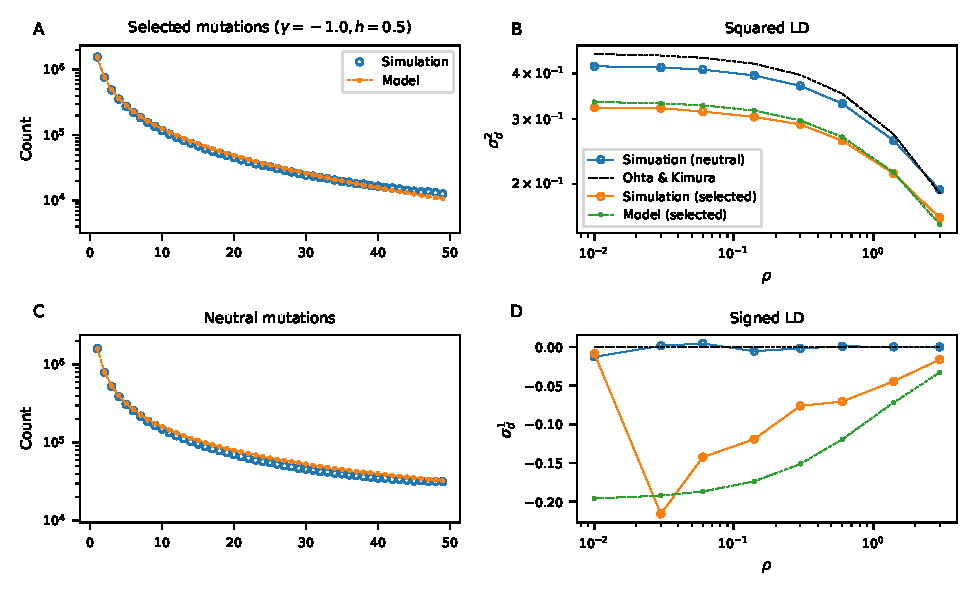
\includegraphics{../figures/bgs_gamma_-1.0_h_0.5_n_50}
    \caption{
        \textbf{Background selection with slightly deleterious mutations.}
        Using an individual-based forward simulator \citep{Thornton2019-qc}, I
        simulated many replicates of 1Mb regions with a high mutation rate of
        selected mutations (see Section~\ref{sec:bgs} for details). Here,
        many linked additive weakly selected mutations slightly distort the
        SFS for both (A) selected and (C) neutral mutations.
        (B) In this scenario of background selection, \(\sigma_d^2\)
        is reduced relative to two-locus expectations without linked selection.
        (D) Hill-Robertson interference effects are slightly diminished, with
        \(\sigma_d^1\) not as strongly negative as expected without additional
        linked selected mutations.
    }
    \label{fig:bgs1}
\end{figure}

\begin{figure}[ht!]
    \centering
    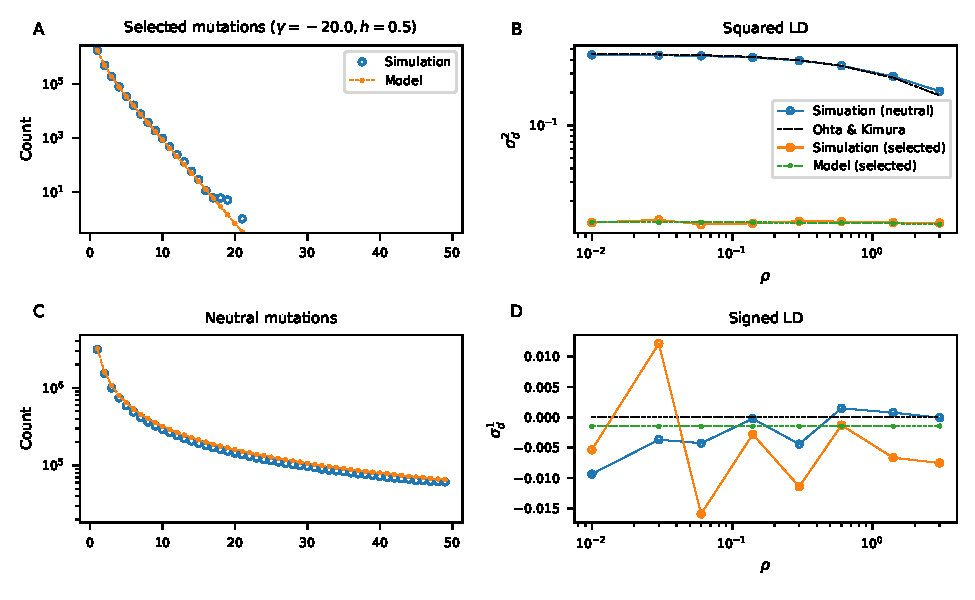
\includegraphics{../figures/bgs_gamma_-20.0_h_0.5_n_50}
    \caption{
        \textbf{Background selection with moderately deleterious mutations.}
        In the case of many linked strongly selected additive mutations, neither
        selected nor neutral statistics deviate dramatically from expectations
        for either the SFS (A, C) or two-locus statistics (B, D).
        The SFS from the simulated data matches single-locus expectations.
        LD is also largely unaffected, with \(\sigma_d^2\)
        matching expectations and \(\sigma_d^1\) fluctuating near zero as expected.
    }
    \label{fig:bgs2}
\end{figure}

\begin{figure}[ht!]
    \centering
    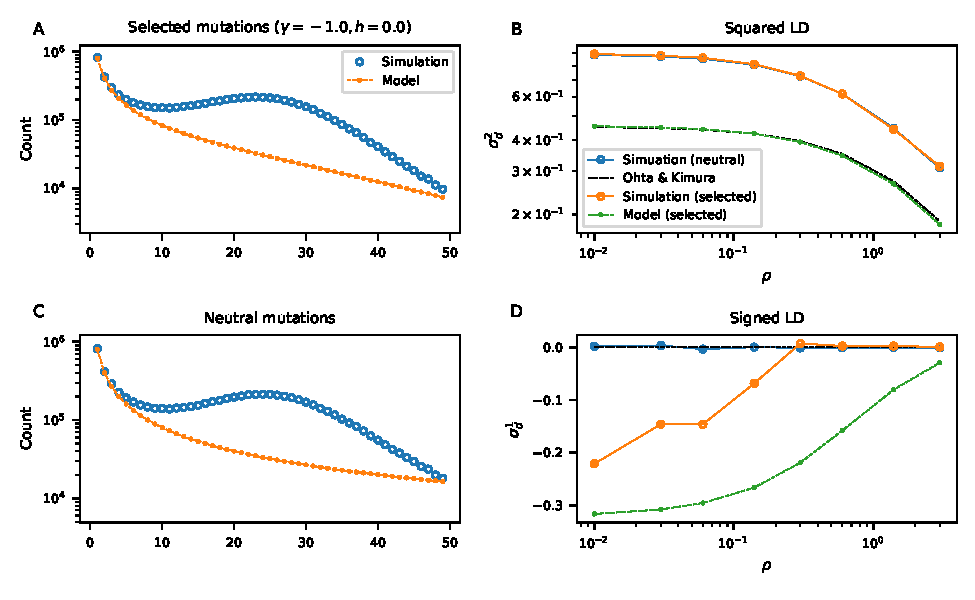
\includegraphics{../figures/bgs_gamma_-1.0_h_0.0_n_50}
    \caption{
        \textbf{Associative overdominance due to slightly deleterious recessive mutations.}
        The presence of many linked weakly selected recessive mutations can cause
        measures of diversity to have large increases over single- and two-locus
        expectations. The SFS for both selected (A) and neutral (C) mutations both show
        a very large excess of common variants (note the log scale), and \(\sigma_d^2\)
        decay curves (B)
        are also increased over two-locus expectations for both classes of mutations.
        (D) \(\sigma_d^1\) remains 0 for neutral mutations and is not as strongly
        negative for pairs of selected mutations due to interference from linked selected
        mutations.
    }
    \label{fig:bgs3}
\end{figure}

\begin{figure}[ht!]
    \centering
    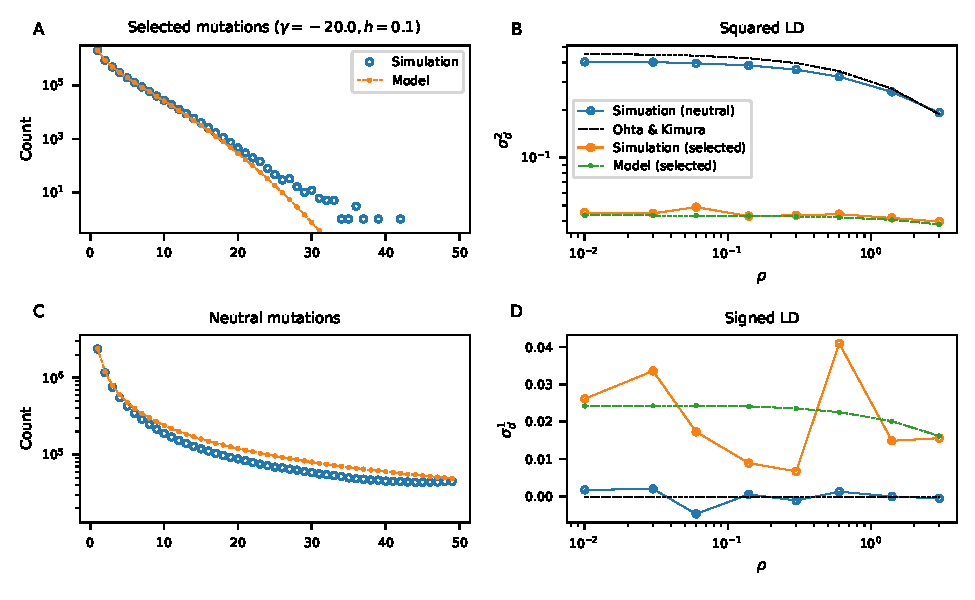
\includegraphics{../figures/bgs_gamma_-20.0_h_0.1_n_80}
    \caption{
        \textbf{Background selection with moderately deleterious recessive mutations.}
        More strongly deleterious recessive mutations do not show as dramatic of
        deviations from expectations as the case of weakly deleterious recessive
        mutations (Fig.~\ref{fig:bgs3}.
        (A) We observe more selected mutations at higher frequencies than expected,
        and (C) the neutral SFS is reduced below single-locus expectations.
        (B, D) LD is also only weakly distorted from
        two-locus expectations. Notably, we see positive LD for strongly
        deleterious recessive mutations (which matches between
        simulations and expectations),
        as previously predicted in \citet{Roze2021-cf}.
    }
    \label{fig:bgs4}
\end{figure}

\begin{figure}[ht!]
    \centering
    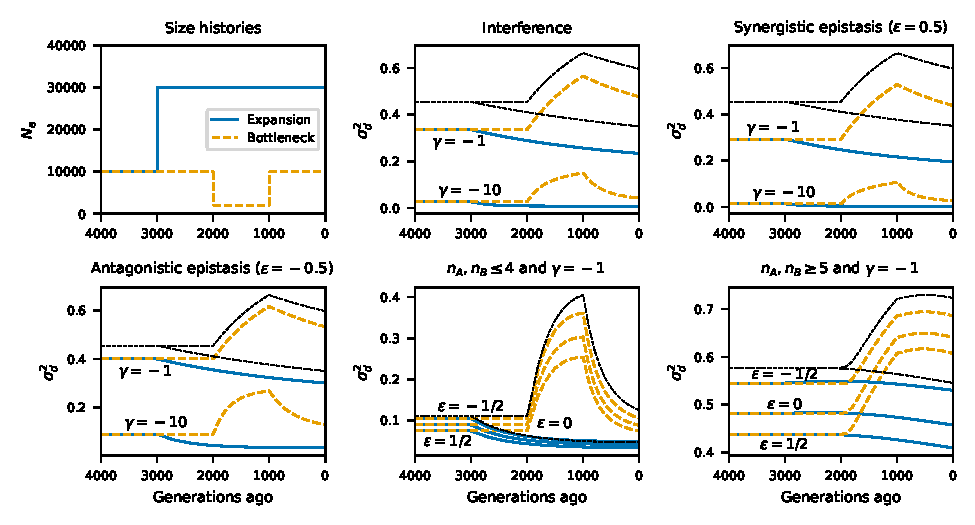
\includegraphics{../figures/demog_bottle_expand.sd2}
    \caption{
        \textbf{Time series of squared LD under bottleneck 
        and expansion histories with epistasis.}
        Bottlenecks increase \(\sigma_d^2\) (squared LD),
        while expansions tend to decrease squared LD.
        Black dashed lines show neutral expectations.
        (A) The simulated size histories. (B-F) Blue solid lines
        are expected squared LD under the expansion model, and gold
        dashed lines are squared LD under the bottleneck/recovery model.
        (B-D) Expectations are computed over all allele frequencies.
        (E) Expected squared LD between uncommon variants, with $n_A$
        and $n_B \leq 4$, in a sample size of 50 haploid copies.
        (F) Expected LD squared LD between common variants
        $p_A, p_B \gtrsim 10\%$.
    }
    \label{fig:toy_sd2}
\end{figure}

\begin{figure}[ht!]
    \centering
    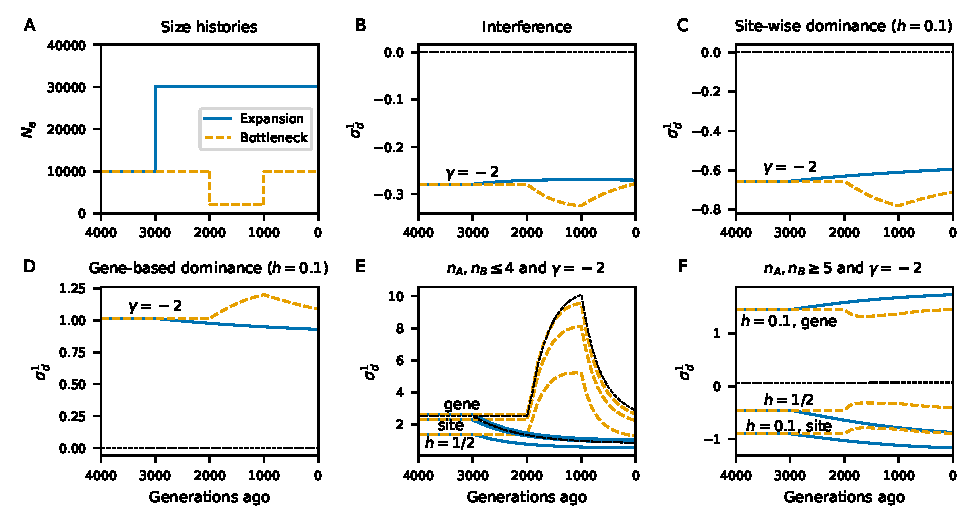
\includegraphics{../figures/demog_bottle_expand.dominance}
    \caption{
        \textbf{Time series of signed LD under bottleneck 
        and expansion histories with dominance.}
        Gene-based dominance, unlike site-wise dominance effects, can cause
        large positive signed LD, similar to compensatory mutations or
        antagonistic epistasis.
        (A) The simulated size histories.
        (B-D) Signed LD computed from pairs of mutations
        across all allele frequencies.
        (E, F) In general, common variants are more
        stable under population size changes than rare variants.
        Dashed lines show neutral expectations.
    }
    \label{fig:toy_dom}
\end{figure}

\begin{figure}[ht!]
    \centering
    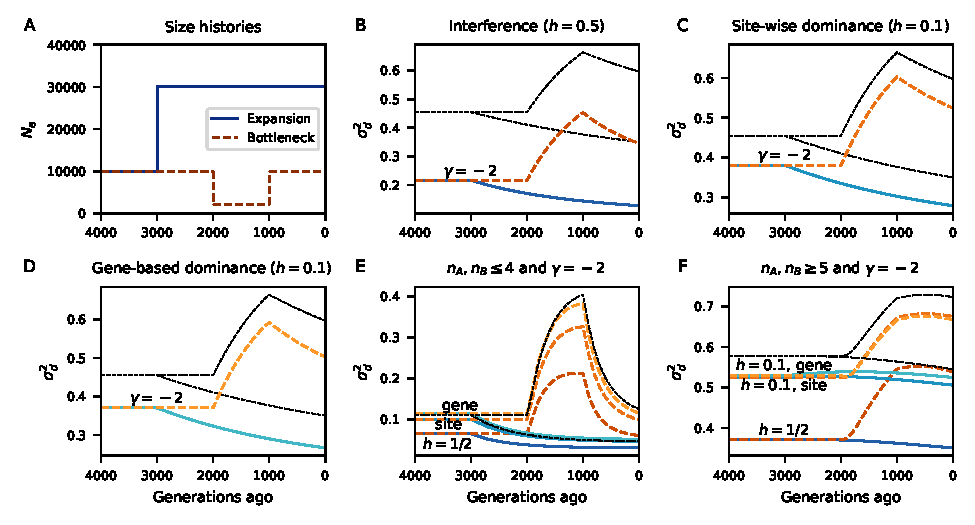
\includegraphics{../figures/demog_bottle_expand.dominance.sd2}
    \caption{
        \textbf{Time series of squared LD under bottleneck 
        and expansion histories with dominance.}
        Similar to the cases with epistasis, bottlenecks tend to increase
        \(\sigma_d^2\) and expansions decrease squared LD.
        (A) The simulated size histories.
        (B-D) Squared LD computed from pairs of mutations at all allele frequencies.
        (E, F) Squared LD computed from uncommon ($<10\%$) and common ($\gtrsim 10\%$)
        mutations.
        Dashed lines show neutral expectations.
    }
    \label{fig:toy_dom_sd2}
\end{figure}

\begin{figure}[ht!]
    \centering
    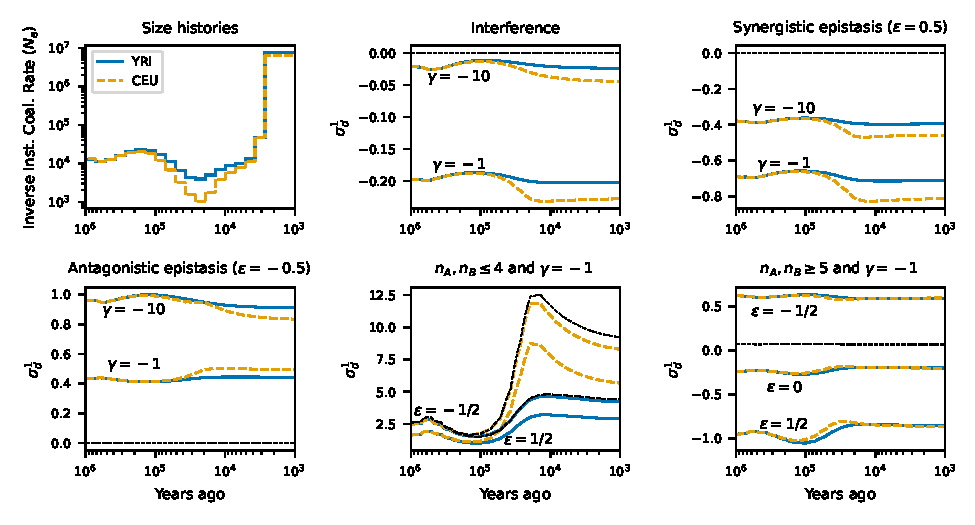
\includegraphics{../figures/demog_YRI_CEU}
    \caption{
        \textbf{Time series of signed LD under inferred models of human population
        size history with with epistasis.}
        (A) Size histories inferred using Relate \citep{Speidel2019-nj}.
        (B-F)
        Similar to the instantaneous size changes in the toy models
        (Figure~\ref{fig:toy}), bottlenecks tend to make signed LD more extreme.
        However, in the case of strong selection and antagonistic epistasis (D),
        the CEU \(\sigma_d^1\) trajectory decreases relative to the YRI
        trajectory, showing that non-constant demographic history and epistasis can
        have complicated interactions.
        (E, F) Again, statistics for rare variants fluctuate more rapidly
        than common variants.
        Dashed lines show neutral expectations.
    }
    \label{fig:relate}
\end{figure}

\begin{figure}[ht!]
    \centering
    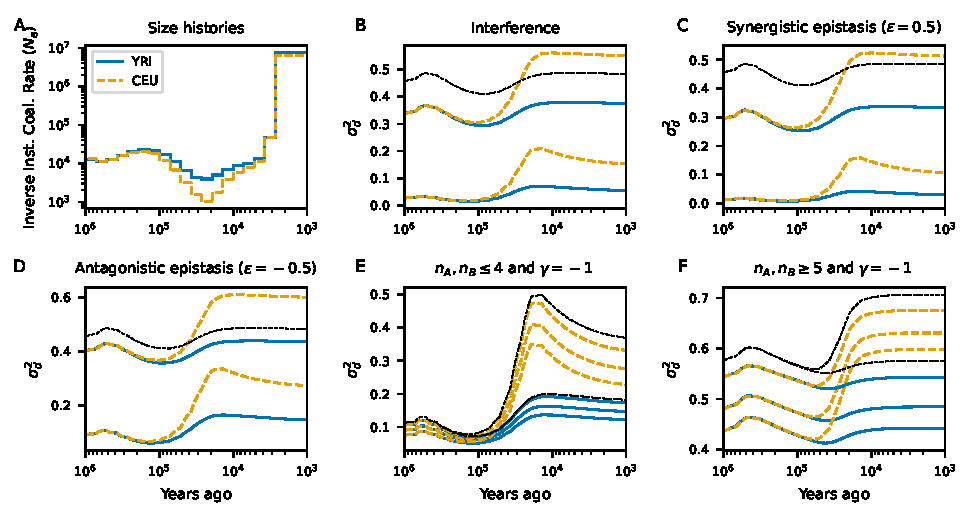
\includegraphics{../figures/demog_YRI_CEU.sd2}
    \caption{
        \textbf{Time series of squared LD under inferred models of human population
        size history with with epistasis.}
        (A) Inferred size histories used in simulations.
        (B-D)
        Size reductions, such as bottlenecks in the recent past of Eurasian populations,
        increase squared LD.
        (E, F) Uncommon and common variants can show strikingly different behaviors
        under size change histories, here showing trajectories under the three
        epistasis models from panels B-D.
        Dashed lines show neutral expectations.
    }
    \label{fig:relate_sd2}
\end{figure}

\begin{figure}[ht!]
    \centering
    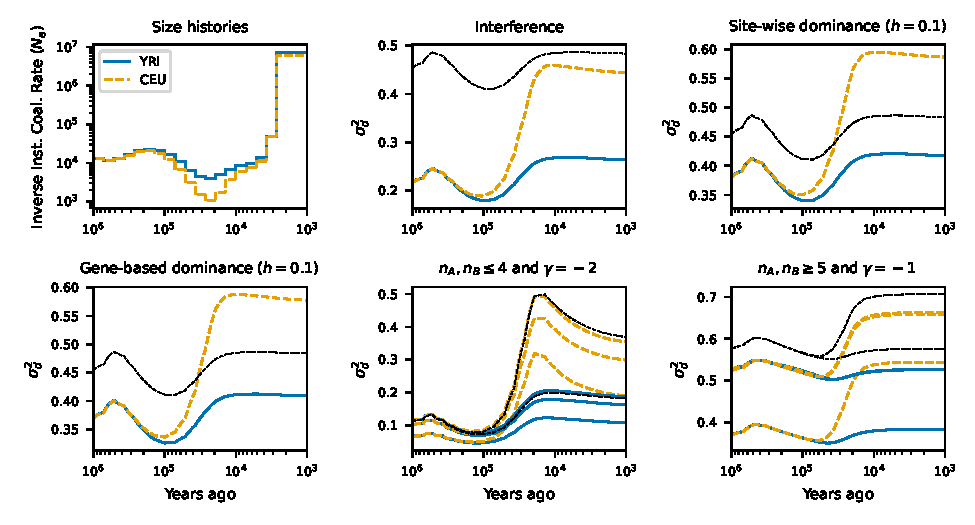
\includegraphics{../figures/demog_YRI_CEU.dominance.sd2}
    \caption{
        \textbf{Time series of squared LD under inferred models of human population
        size history with with dominance.}
        (A) Inferred size histories used in simulations.
        (B-D)
        Again, bottlenecks increase squared LD relative to populations that did
        not experience such strong size reductions in their history.
        (E, F) Uncommon and common variants can show strikingly different behaviors
        under size change histories, here showing trajectories under the three
        dominance models from panels B-D.
        Dashed lines show neutral expectations.
    }
    \label{fig:relate_dom_sd2}
\end{figure}

\begin{figure}[ht!]
    \centering
    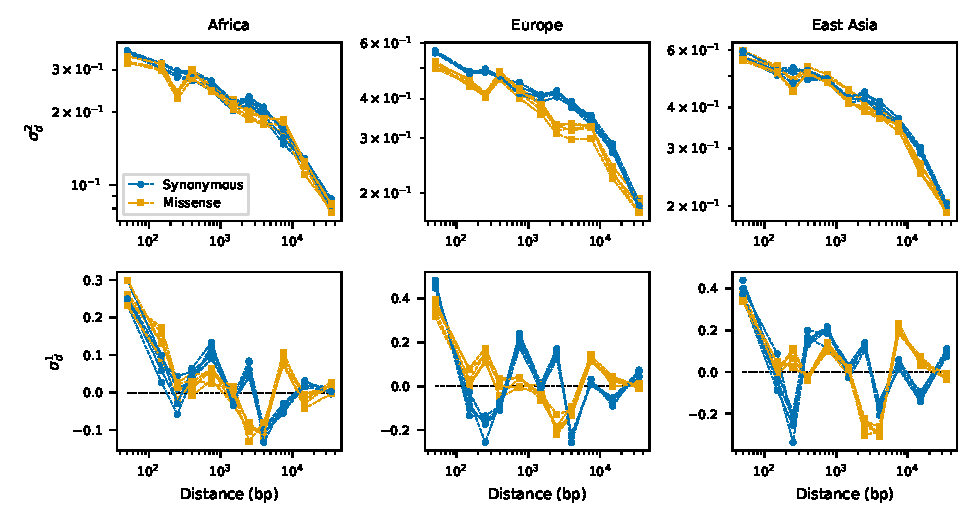
\includegraphics{../figures/ld_decay_gene_wide}
    \caption{
        \textbf{LD decay for pairs of synonymous and missense mutations
        in the same gene.}
        When taking gene-wide averages of LD, there are no obvious differences
        between the LD decay curves of synonymous and missense mutations.
        Each panel contains five LD decay curves for each mutation class, one for
        each \citet{1000_Genomes_Project_Consortium2015-zq} population in the
        continental groupings. Shared demographic history leads to strong
        correlation in statistics between populations in the same continental
        groups.
    }
    \label{fig:LDgene}
\end{figure}

\begin{figure}[ht!]
    \centering
    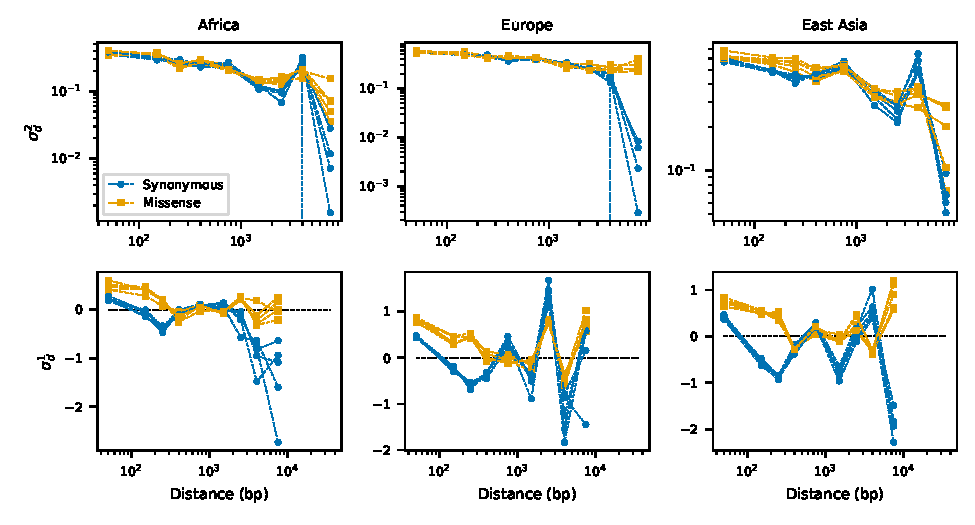
\includegraphics{../figures/ld_decay_in_domain}
    \caption{
        \textbf{LD decay for pairs of synonymous and missense mutations
        that fall inside the same domain.}
        At short distances between SNPs that both fall within sthe same conserved
        annotated domain, missense mutations show consistently
        larger signed LD than synonymous variants. This may be caused by
        antagonistic epistasis or compensatory effects between pairs of
        nearby missense mutations.
    }
    \label{fig:LDwithin}
\end{figure}

\begin{figure}[ht!]
    \centering
    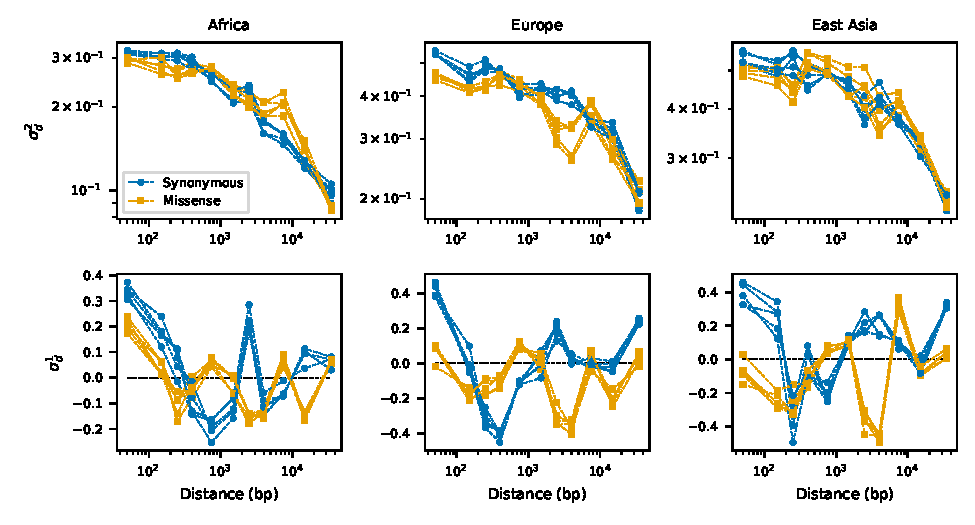
\includegraphics{../figures/ld_decay_outside_domains}
    \caption{
        \textbf{LD decay for pairs of synonymous and missense mutations
        outside of domains.}
        Outside of conserved domains,
        missense mutations have reduced signed LD at short distances
        compared to synonymous mutations,
        opposite the pattern observed within domains (Figure~\ref{fig:LDwithin}).
        This pattern is consistent with Hill-Robertson interference between
        missense mutations outside of conserved elements.
    }
    \label{fig:LDoutside}
\end{figure}

\begin{figure}[ht!]
    \centering
    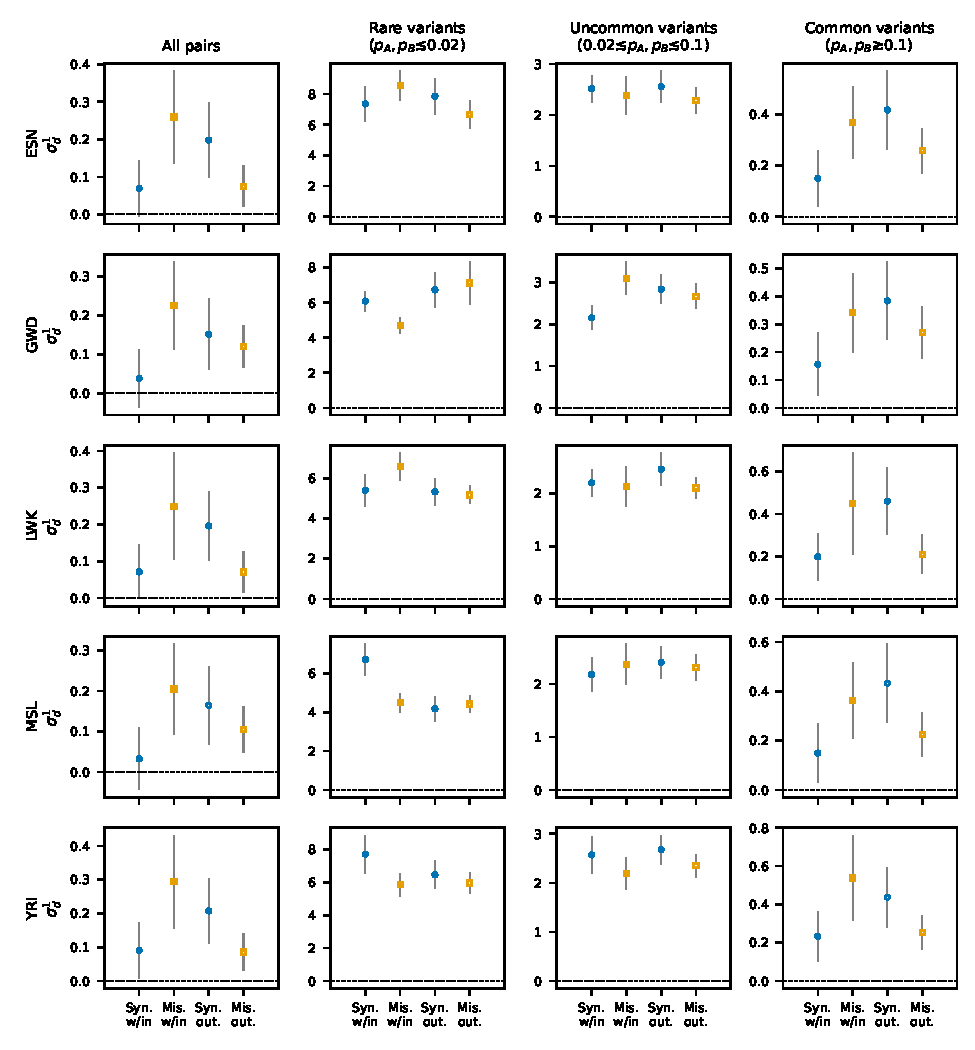
\includegraphics{../figures/data_domains_afr}
    \caption{
        \textbf{LD for pairs of synonymous and missense mutations within the
        same domain and outside domains at matched distances.}
        Showing the five populations in the Thousand Genomes African group.
        We observe increased LD between missense mutations within domains,
        but decreased LD outside of domains at matched distances. This pattern
        holds when conditioning on non-rare variation (\(n_A, n_B \geq 9\),
        MAF \(\gtrsim 0.05\)).
    }
    \label{fig:domainsAFR}
\end{figure}

\begin{figure}[ht!]
    \centering
    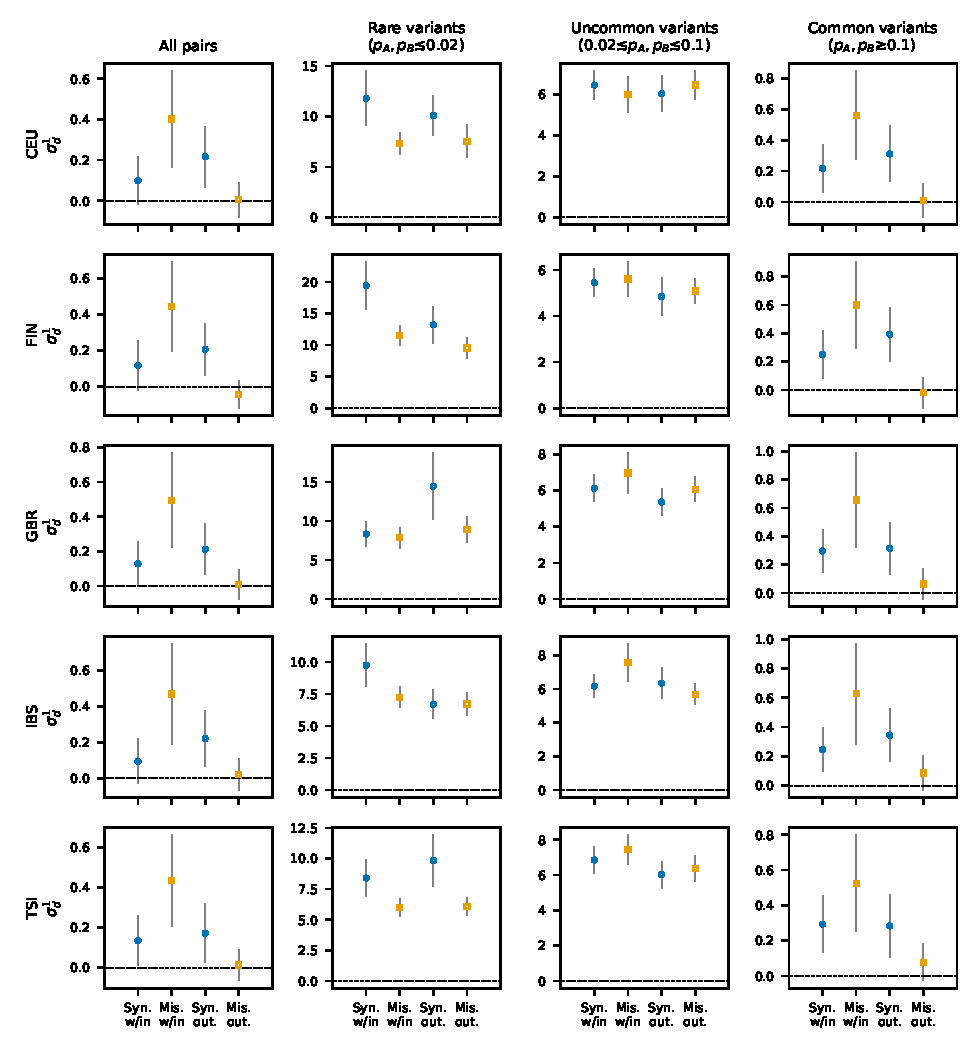
\includegraphics{../figures/data_domains_eur}
    \caption{
        \textbf{LD for pairs of synonymous and missense mutations within the
        same domain and outside domains at matched distances.}
        Showing the five populations in the Thousand Genomes European group.
        We again observe increased LD between missense mutations within domains,
        but decreased LD outside of domains at matched distances. And again,
        this pattern holds when conditioning on non-rare variation
        (\(n_A, n_B \geq 9\), MAF \(\gtrsim 0.05\)).
    }
    \label{fig:domainsEUR}
\end{figure}

\begin{figure}[ht!]
    \centering
    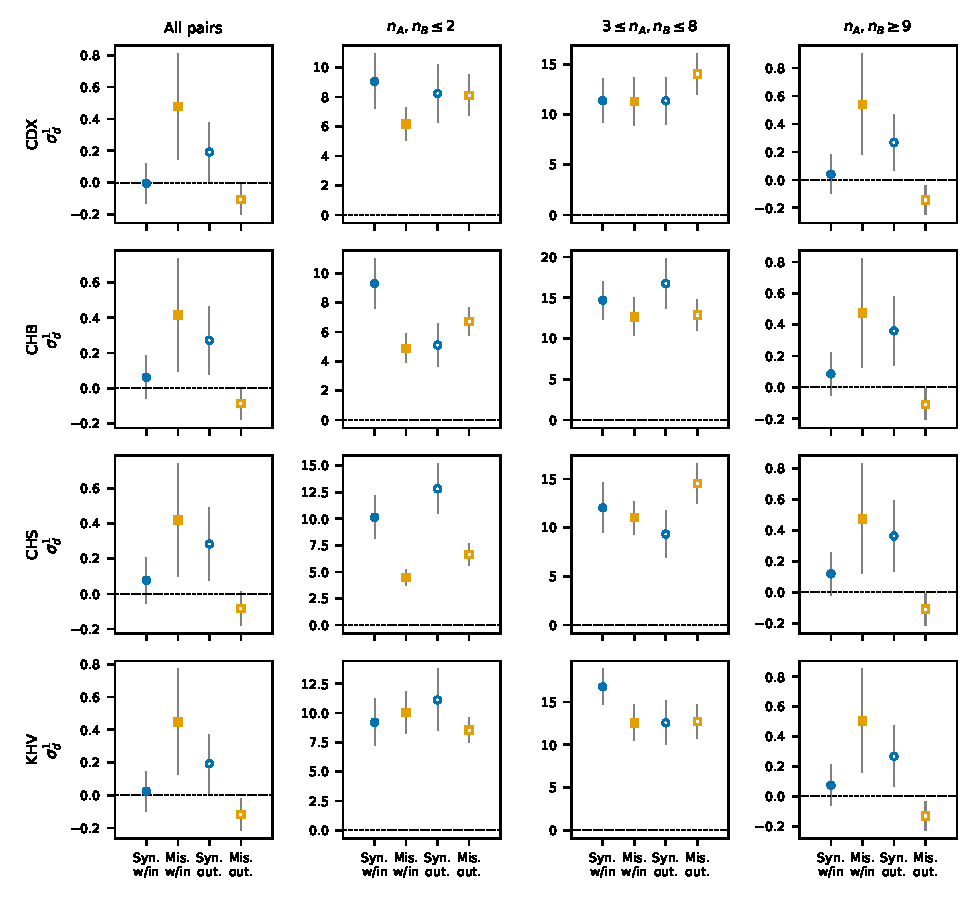
\includegraphics{../figures/data_domains_eas}
    \caption{
        \textbf{LD for pairs of synonymous and missense mutations within the
        same domain and outside domains at matched distances.}
        Showing the five populations in the Thousand Genomes East Asian group.
        As with the African and European data,
        we observe increased LD between missense mutations within domains,
        but decreased LD outside of domains at matched distances. And again,
        this pattern holds when conditioning on non-rare variation
        (\(n_A, n_B \geq 9\), MAF \(\gtrsim 0.05\)).
    }
    \label{fig:domainsEAS}
\end{figure}

\begin{figure}[ht!]
    \centering
    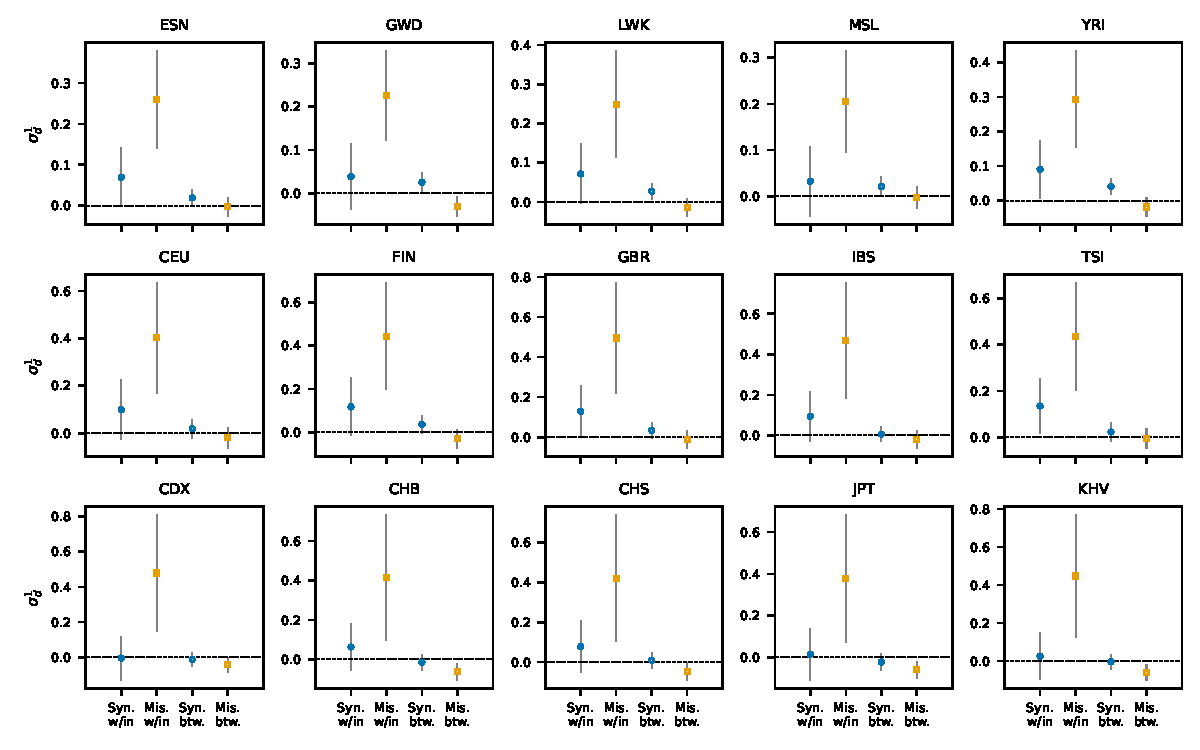
\includegraphics[width=\textwidth]{../figures/data_within_between}
    \caption{
        \textbf{LD for pairs of synonymous and missense mutations both within the same
        domain and in differing domains.}
        In each panel (one for each population), the left two data points show signed
        LD between mutations that fall within the same domain, and the right two
        data points show signed LD between mutations falling within domains but
        in \emph{different} domains within the same protein-coding gene. Distances
        are not matched between these data classes (as between-domain pairs are
        typically more distant than within-domain pairs). Increased LD between
        missense mutations is only observed for pairs of mutations within the same
        domain, but not between domains.
    }
    \label{fig:between_domains}
\end{figure}

\begin{figure}[ht!]
    \centering
    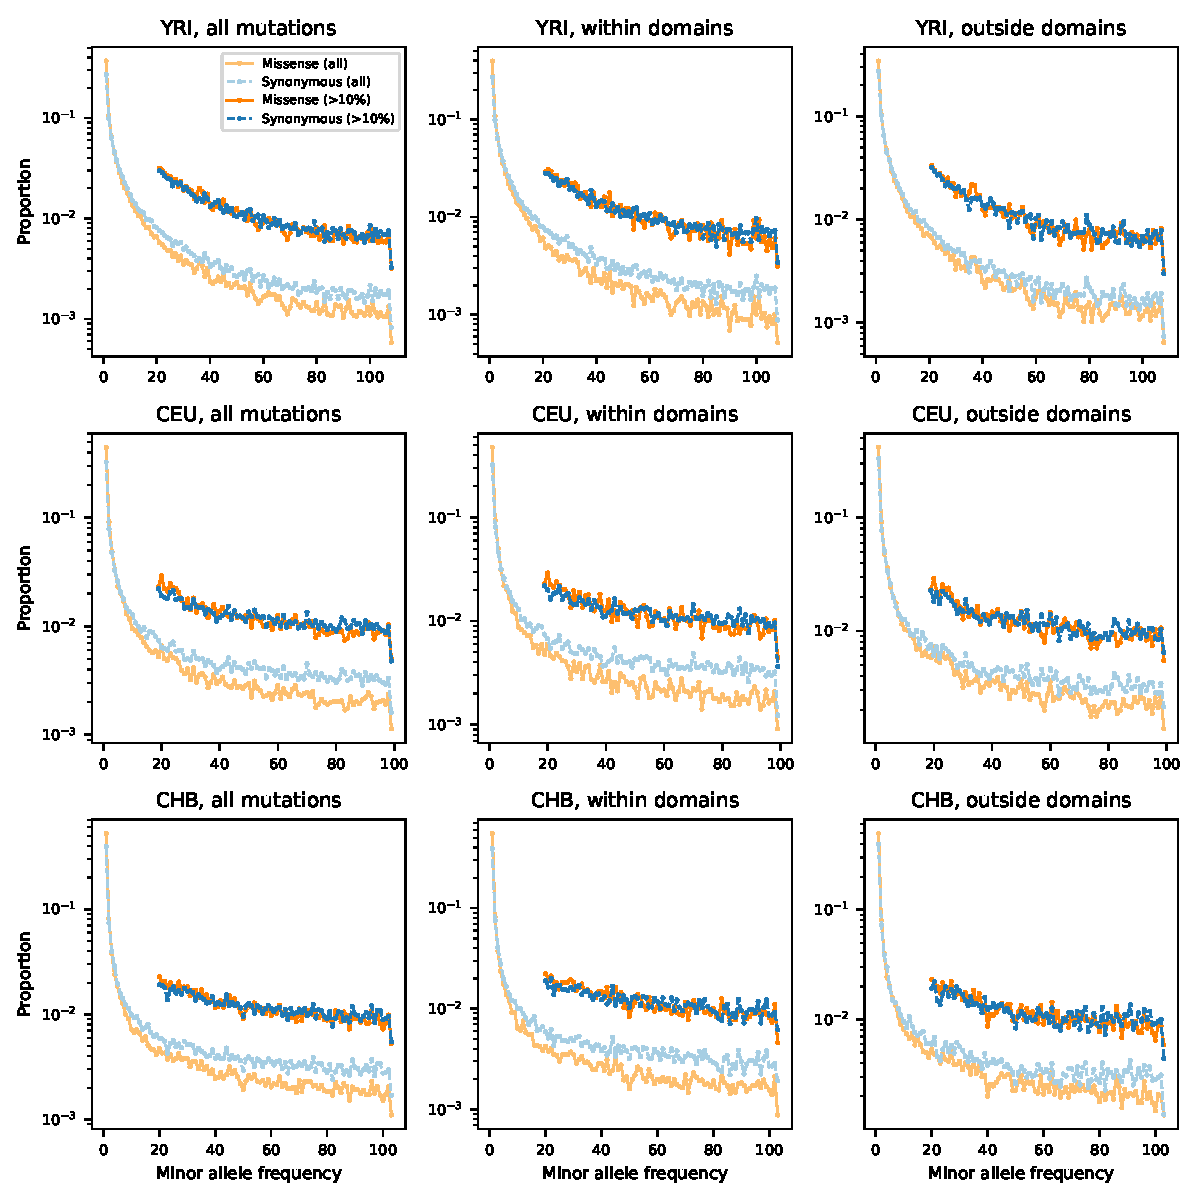
\includegraphics[width=\textwidth]{../figures/SFS_proportions}
    \caption{
        \textbf{SFS for common missense and synonymous variants.}
        The full SFS (considering variants at all observed allele frequencies) is
        skewed toward low frequencies for missense variants compared to synonymous
        variants (shown in light colors). Tajima's $D$ is considerably more negative
        for missense variants than synonymous variants for missense variants, whether
        conditioning on mutations within annotated elements or outside
        (Table~\ref{tab:tajimasD}). However, the SFS for common variants (with
        observed MAF $\geq 10\%$) are similar between missense and synonymous variants
        for each partition of the data. Thus, the excess of positive signed LD for
        common variants within annotated domains is likely not to be driven by
        subtle differences in allele frequencies between missense and synonymous
        classes.
    }
    \label{fig:sfs_proportions}
\end{figure}

\begin{figure}[ht!]
    \centering
    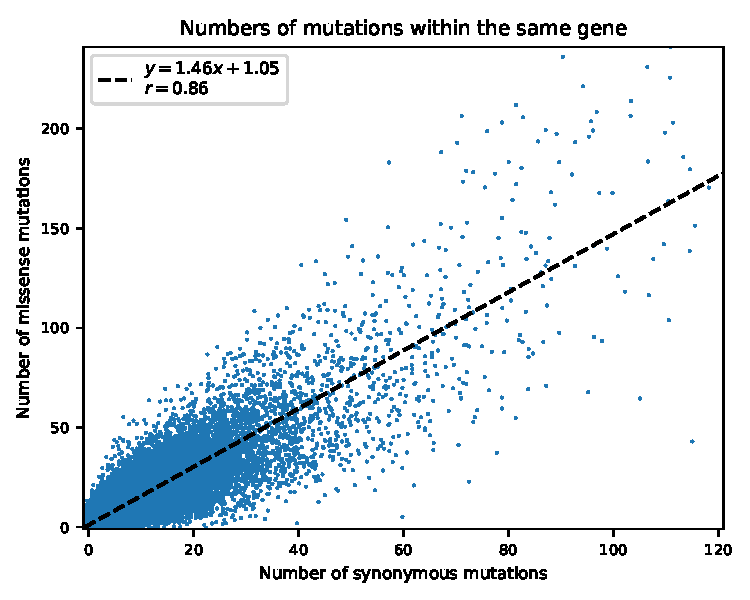
\includegraphics{../figures/mutations_in_genes}
    \caption{
        \textbf{Correlation between numbers of missense and synonymous mutations
        within each gene.}
        Human genes have different sizes and sequence content, so they may differ in the
        numbers of missense and synonymous mutations observed within them.
        The number of missense mutations within a gene is predicted well by
        the number of synonymous mutations (\(r=0.86\)).
    }
    \label{fig:mutCorrGene}
\end{figure}

\begin{figure}[ht!]
    \centering
    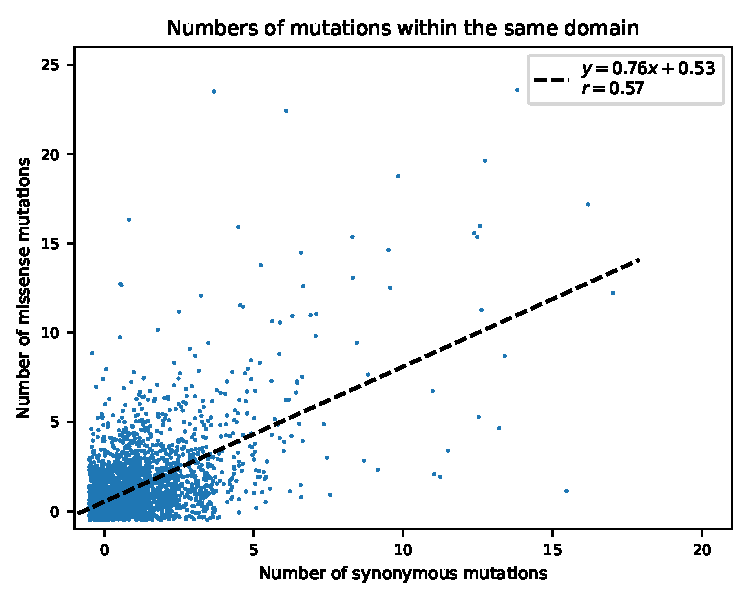
\includegraphics{../figures/mutations_in_domains}
    \caption{
        \textbf{Correlation between numbers of missense and synonymous mutations
        within each annotated domain.}
        Domains are typically much smaller than the average gene-size, and while
        the number of synonymous mutations within a domain is moderately predictive
        of the number of missense mutations within the same domain (\(r=0.57\)),
        this correlation is weaker than the correlation in gene-wide mutation
        counts (Figure~\ref{fig:mutCorrGene}).
    }
    \label{fig:mutCorrDomain}
\end{figure}

\begin{figure}[ht!]
    \centering
    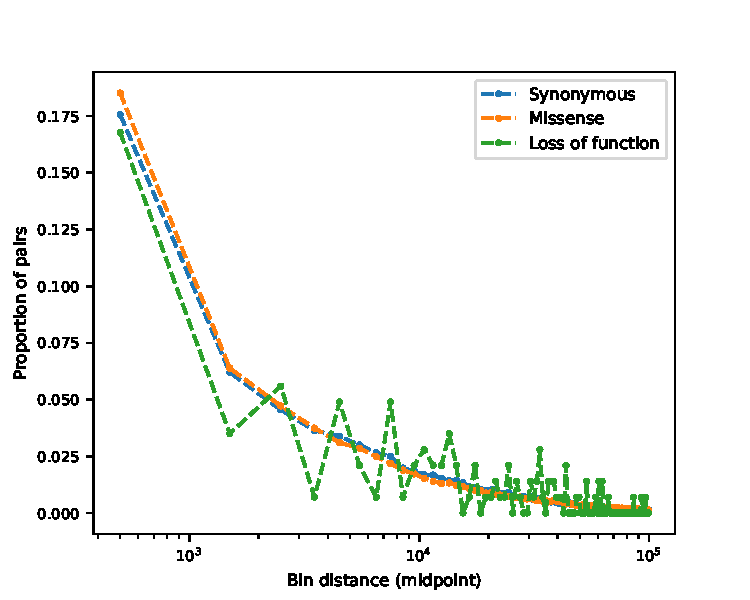
\includegraphics{../figures/mutation_class_distances}
    \caption{
        \textbf{Distances between mutation pairs for different classes of variants.}
        Despite different mutation rates between classes of mutations, the
        proportions of pairs of mutations at given distances are similar.
        Missense mutations, which have the highest mutation rate within genes,
        have slightly more pairs of mutations at close distances than synonymous,
        with loss of function mutations, which have the lowest mutation rate within
        genes, have the fewest pairs at short distances.
    }
    \label{fig:mutDistances}
\end{figure}

\begin{figure}[ht!]
    \centering
    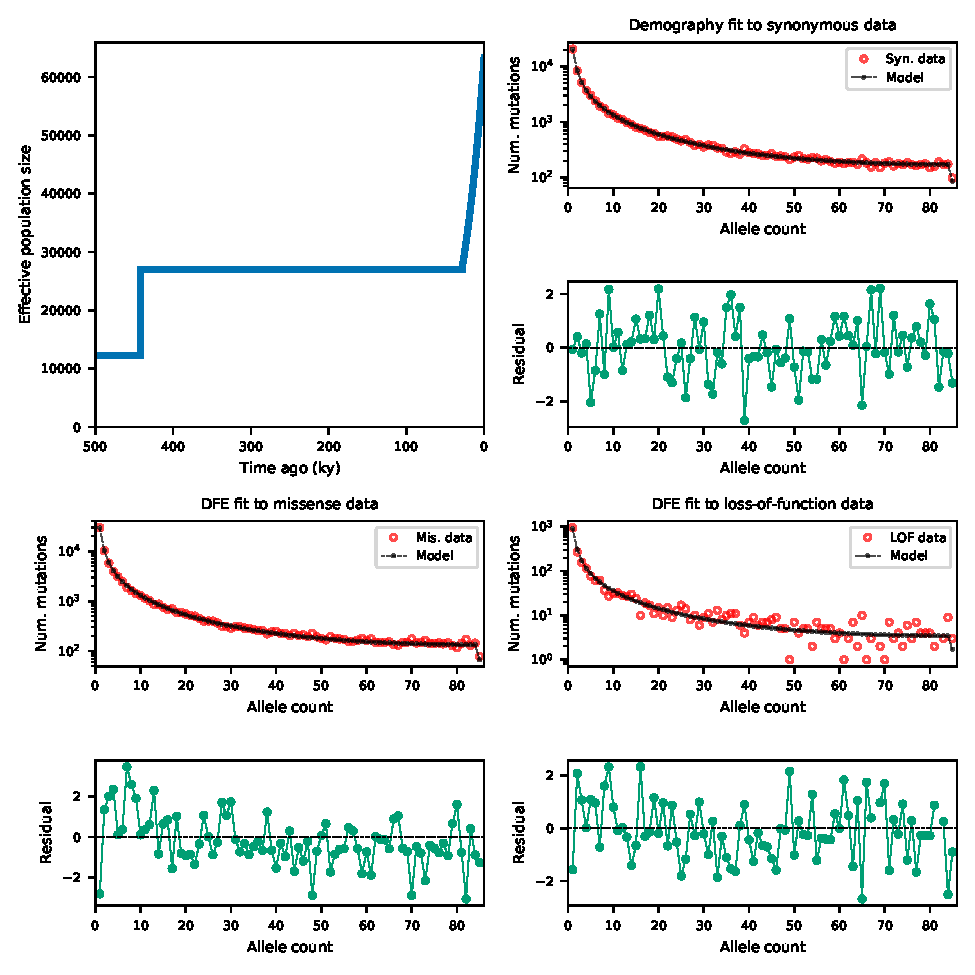
\includegraphics{../figures/msl_demography_dfes}
    \caption{
        \textbf{Demography and DFE for MSL.} A demographic model was fit to
        the folded synonymous SFS, and DFEs were fit to missense and loss-of-function
        SFS. Shown here are DFEs fit with \(h=0.5\). See Table \ref{tab:msldfe} for
        inferred best-fit parameters.
    }
    \label{fig:msldemogdfe}
\end{figure}

\begin{figure}[ht!]
    \centering
    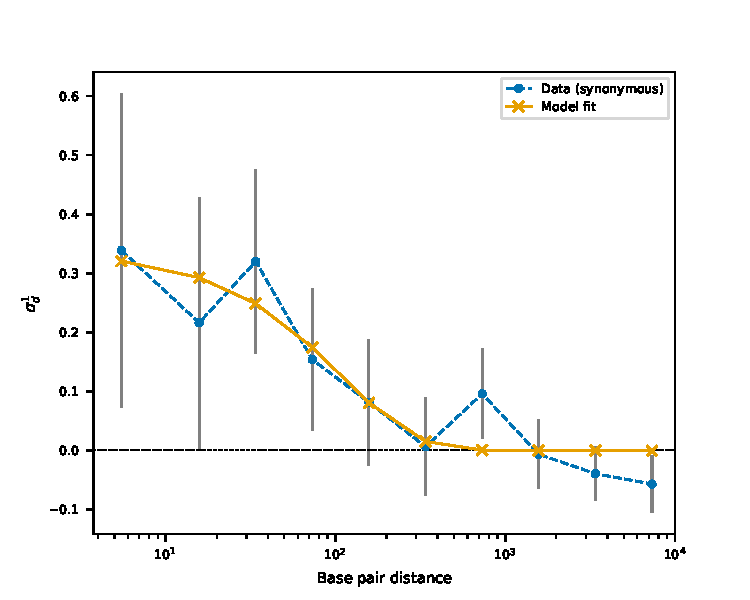
\includegraphics{../figures/msl_mnms.v2}
    \caption{
        \textbf{Optimization of fraction of new mutations arising via
        multinucleotide mutations by distance.} 
        A simple exponential function was fit to LD decay of synonymous mutations,
        to describe the probability that a given mutation event is a multinucleotide
        mutation event that spontaneously gives rise to a pair of perfectly linked
        mutations at count \(1/2N\).
        Fitting \(Ae^{-\lambda d}\) to mutations (see Section~\ref{sec:mnm}),
        the best fit parameters across all recombination rates
        tested were \(A=2.4\times10^{-5}\) and \(\lambda=0.0092\), showing that even
        small rates of multinucleotide mutation events can cause increased signed
        LD at short distances.
    }
    \label{fig:mslmnms}
\end{figure}

\end{document}
